%% 美赛模板:正文部分

\documentclass[12pt]{article}  % 官方要求字号不小于 12 号,此处选择 12 号字体

% 本模板不需要填写年份,以当前电脑时间自动生成
% 请在以下的方括号中填写队伍控制号
\usepackage[2417377]{easymcm}  % 载入 EasyMCM 模板文件
\problem{A}  % 请在此处填写题号
%\usepackage{mathptmx}  % 这是 Times 字体,中规中矩 
\usepackage{mathpazo}  % 这是 COMAP 官方杂志采用的更好看的 Palatino 字体,可替代以上的 mathptmx 宏包

\usepackage{threeparttable}

\title{The Role of Variable Sex Differentiation Ratios in Populations and Ecosystems}  % 标题

% 如需要修改题头(默认为 MCM/ICM),请使用以下命令(此处修改为 MCM)
%\renewcommand{\contest}{MCM}

%此处用于给公式编号
\makeatletter
\@addtoreset{equation}{section}
\makeatother
\renewcommand{\theequation}{\arabic{section}-\arabic{equation}}

% 文档开始
\begin{document}

% 此处填写摘要内容
\begin{abstract}
As one of the few remaining jawless vertebrate fish-like organisms, lamprey is a highly regarded subject in contemporary research. Additionally, lamprey exhibits sexless larvae and differentiates sexes based on environmental food availability, which holds significant importance for studying species' sex ratios in relation to population size, resource availability, and ecological chains.

For Problem 1, we begin with a basic two-sex model and explore the relationship between fixed male differentiation rates and environmentally available food. Considering that species cannot grow indefinitely, we introduce a logistic model with a reproduction rate equation to regulate population growth. Subsequently, we examine the variable male differentiation rates by normalizing it within the range of 0.56 to 0.78 as per question requirements to establish the connection between male differentiation rates and current resource availability. Variable male differentiation rates enable lamprey populations to efficiently utilize resources which results in fewer resource availability in the environment.

For Problem 2, our study expands into the food chain by incorporating the Lotka-Volterra predation equation and add prey to the food chain, while considering varying predation abilities among male and female lampreys. This successful modeling allows us to analyze phase relationships within the food chain system. We discover that populations with variable male differentiation rates can occupy more resources within an ecosystem, providing them with an advantage; However, this also raises their risk that extinction of one sex results in the extinction of the whole population.

For Problem 3, we introduce the Lyapunov exponent from the field of automatic control to quantitatively measure the stability of the entire system. We then add competitors and predators to form a food web based on the previous one, and discover that varying male differentiation rates results in increased ecosystem stability.

For Problem 4, we take into account that organisms reproduce discretely and therefore used a metacellular automaton based on differential equations for discrete simulation of our model. Ultimately, we find that variable differentiation ratio in lamprey leads to greater stability among other populations.

Eventually, stability and sensitivity analysis are conducted on the model. In the cellular automaton, the initial distribution of the population is random and has no significant effect on the final results. As for the factor that affects the model, namely the mortality rate, we find that its alteration noticeably influences the stability of the ecosystem, indicating good model sensitivity.

    % 美赛论文中无需注明关键字。若您一定要使用,
    % 请将以下两行的注释号 '%' 去除,以使其生效
    \vspace{5pt}
    \textbf{Keywords}: Sex differentiation ratio, Lamprey, Lotka–Volterra equation, Lyapunov's theorem, Logistic function, Cellular Automata.

\end{abstract}

\maketitle  % 生成 Summary Sheet
\tableofcontents  % 生成目录

% 正文开始
\section{Introduction}
\subsection{Problem Background}
A population that is necessarily dependent on reproduction for its development and continuation. Based on sexual reproduction, the growth rate of a population is greatly influenced by the sex ratio. Therefore, although many species exhibit a 1:1 sex ratio at birth, species tend to deviate from an even sex ratio in order to adapt to their environment and continue their populations. This is known as adaptive sex ratio variation.\cite{1} The lamprey is one such typical species.

However, the role of the lamprey is complex. For some lake habitats, it is a parasite that is harmful to the ecosystem, and we want to reduce its reproduction; but at the same time, it is a source of food in some parts of the world, and we want to promote its reproduction.\cite{2} Therefore, we address these questions by studying the pros and cons of the ability to alter their sex ratio based on resource availability, modeling their relationship with growth rates, and studying their impact on other species in the ecosystem.
\begin{figure}[htbp]
	\centering
	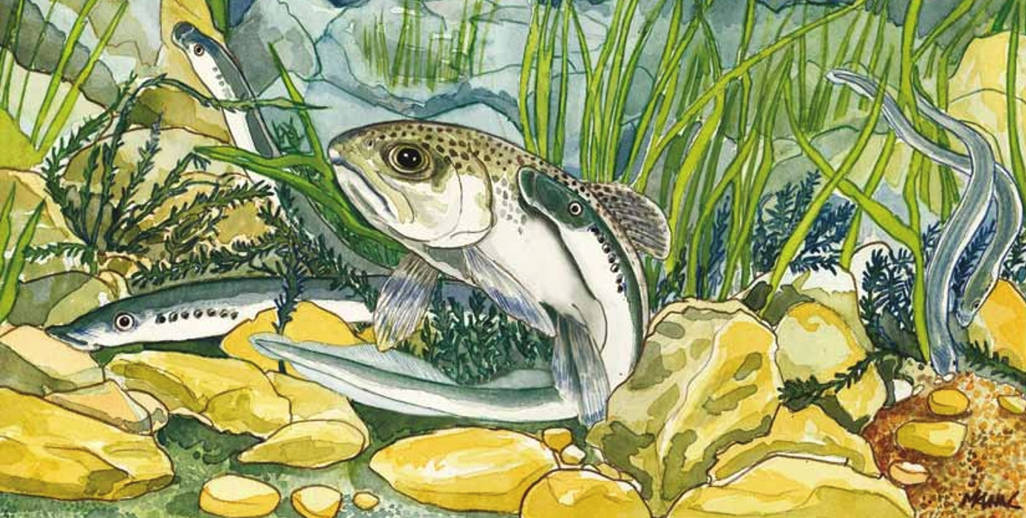
\includegraphics[width=.6\textwidth]{a fish with lamprey.jpg}
	\caption{a fish with lampreys}\label{a fish with lampreys}
\end{figure}
\subsection{Restatement of the Problems}

\begin{itemize}
	\item Develop and examine a model to provide insights into the impact on the larger ecological system when the population of lampreys can alter its sex ratio
	\item Evaluate the advantages and disadvantages of the ability to change sex ratios for the population itself and for the external ecosystem under the same resource availability conditions, taking into account the modeling of Question 1
	\item Study the impact of sex ratio on ecosystem stability, specifically speaking,to evaluate the impact on ecosystems by considering the influence of changing population sex ratios on other populations on the basis of previous models
	\item Developing a model to describe the relationship between lampreys and its parasites, competitors and predators study whether ecosystems with changing population sex ratios can provide advantages to other species in the ecosystem such as parasites, competitors and predators
\end{itemize}

\subsection{Overview of Our work}
In order to find the relationship between sex ratio and environmental availability, we model the dynamics of the population and gradually added predator and parasite interactions to the model, constituting a model of the effect of variable sex ratio on the ecosystem, and finally, based on the model, we propose the role of sex ratio control for human beings in the ecosystem.

\begin{itemize}
	\item Assumptions are made to reduce complex ecosystems and the interactions within them (e.g., food chain relationships) to plausible resource-pressure relationships, and typical predation and parasitism relationships are included for objective modeling of population changes
	\item Modeling populations. Based on the Logitics model and the population dynamics equation, a sex ratio-environmental availability model is developed to study its effects on the population itself, as well as on the ecosystem
	\item Modeling ecosystem interactions. Based on the Lotka-Volterra equation, predators and parasits are introduced respectively, and the model is improved so that it could describe the interactions of various groups in the ecosystem to study the role of sex ratios, and the Lyapunov’s theorem and Cellular Automata are used to study
	the effects on ecosystem stability\cite{5} and the advantages lamprey population offer to others in the ecosystem
	\item Analyze the strengths and weaknesses of the model and make the conclusions
\end{itemize}

\begin{figure}[!htbp]
	\centering
	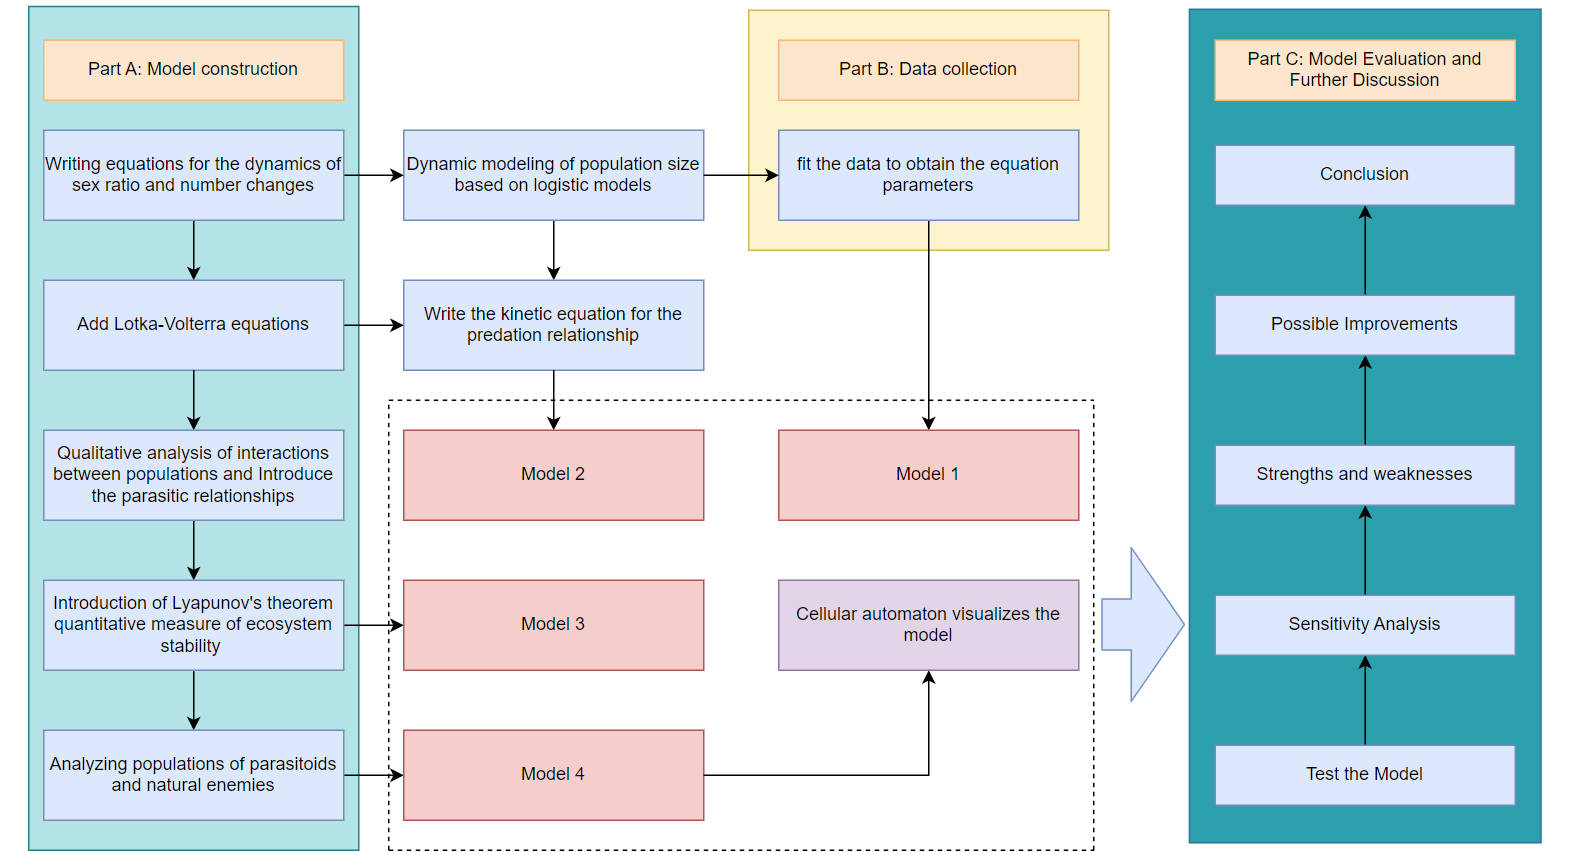
\includegraphics[width=0.88\textwidth]{work.jpg}
	\caption{our work}\label{work}
\end{figure}

\section{Assumptions and Justification}
\begin{itemize}
	\item \textbf{Assumption 1:}
	We assume that the number of producers and the amount of energy produced are constant in this system
	
	$\hookrightarrow$Justification:We only explore the effect of the sex ratio of lamprey on lamprey and the trophic levels above and below the lamprey, and we ignore the secondary effects for the time being.\cite{1}
	\item \textbf{Assumption 2:}
	The growth rate of lamprey is not affected by migration behavior and human activities
	
	$\hookrightarrow$Justification: We consider a spatially large environment, so that the population growth rate will not be changed due to the effect of migration rate.\cite{2}
	\item \textbf{Assumption 3:}
	Male and female lampreys do not differ in their ability to access resources based on age
	
	$\hookrightarrow$Justification:The time period of our study is long enough to determine that the ability of both males and females to access resources is the average of the lamprey's ability to access resources over their lifetime.\cite{3}
	\item \textbf{Assumption 4:}
	Intraspecific competition is ignored and only the effect of interspecific competition is considered
	
	$\hookrightarrow$Justification:Interspecific competition is much stronger than intraspecific competition and is more pronounced in parasitic organisms.\cite{3}

\end{itemize}

\section{Notations}
% 三线表示例
\begin{table}[!htbp]
\begin{center}
\begin{threeparttable}
\caption{Notations}\label{notations}
\begin{tabular}{cl}
	\toprule
	\multicolumn{1}{m{3cm}}{\centering Symbol}
	&\multicolumn{1}{m{12cm}}{\centering Definition}\\
	\midrule
	$N_{F}$&the number of female lamprey\\
	$N_{M}$&the number of male lamprey\\
	$TNL$ &total number of lamprey\\
	$RA$&resource availability\\
	$c$&Population fertility coefficient\\
	$r$ &the growth rate relative to sex ratio\\
	$\alpha$ &the proportion of male in lamprey after sex differentiation\\
	$\beta$ &the decrease rate in relation to number\\
	$\lambda$&The number of viable eggs laid at one time\\
	$\epsilon$&the predation conversion factor\\
	$a$&predatory capacity of lamprey\\
	\bottomrule
\end{tabular}
\small
\textit{Other notations instructions will be given in the text.}
\end{threeparttable}
\end{center}
\end{table}

\section{Model 1: Sex Ratio Resource Consumption Model}
\subsection{Description of Lampreys and the Ecosystems}
We first consider the effect of the sex ratio of lampreys on the availability resource of the system in which they are found. In an ecosystem where the availability resource is $RA$ ideally, let the sex-related reproduction rate of lampreys be $r$, the total number of males in the population be $N_M$, the total number of females $N_F$, and the total number of lampreys $TNL$, and we can obtain the equation:

\begin{equation}\label{eq:4-1}
		TNL = N_{F} + N_{M} 
\end{equation}

In this ecosystem, the growth number of the next generation is always determined by the total number of lampreys in the population now, so we can know:

\begin{equation}\label{eq:4-2}
	\frac{N(t')-N(t)}{t'-t}=\frac{\Delta N}{\Delta t}=\frac{\mathrm{d}N_{M}}{\mathrm{d}t}
\end{equation}

And the $\frac{\mathrm{d}N_{M}}{\mathrm{d}t}$ is determined by the current $r$, $RA$, $N_F$, $N_M$, and we consider the males and females of the progeny separately, so we can get the equation:

\begin{equation}\label{eq:4-3}
\begin{cases}
	\frac{\mathrm{d}N_{M}}{\mathrm{d}t}=F(r,RA,N_{F},N_{M})\
	\\ \\
	\frac{\mathrm{d}N_{F}}{\mathrm{d}t}=G(r,RA,N_{F},N_{M})\\
\end{cases}
\end{equation}

In the equation, obviously, since the species reproduces sexually, the reproduction rate of lampreys is related to the number of male and female lampreys and their ratio, which can be expressed as:

\begin{equation}\label{eq:4-4}
r = \mu(N_{M},N_{F})
\end{equation}

Moreover, since the total amount of resources in a stable ecosystem without considering external influence is always certain, and the population will occupy a certain amount of resources. Therefore, when we consider the impact of the lamprey population on the environmental resources, the remaining resources that are not occupied by the lamprey are the available resources, and it is obvious that the available resources are negatively correlated with the total number of individuals in the lamprey population:

\begin{equation}\label{eq:4-5}
RA = \xi(TNL)
\end{equation}

Therefore, considering the equation (\ref{eq:4-1}) (\ref{eq:4-3}) (\ref{eq:4-4}) and substituting them into (\ref{eq:4-2}), we can know that:

\begin{equation}\label{eq:4-6}
\begin{cases}
	\frac{\mathrm{d}N_{M}}{\mathrm{d}t}=F(N_{F},N_{M})\
	\\  \\
	\frac{\mathrm{d}N_{F}}{\mathrm{d}t}=G(N_{F},N_{M})\\
\end{cases}
\end{equation}

\subsection{Derivation and Modeling the Model}
Here logistic model is introduced and we consider that the rate of reproduction of lamprey is proportional to the environmental availability of resources and also to the reproduction rate, and the rate of mortality is proportional to the number of lampreys with a mortality coefficient $\beta$.

Since lamprey pups do not differentiate between the sexes until adulthood, sex can be affected by environmental factors. Now assume for a moment that the environmental conditions do not change over a short period of time, so let the male differentiation rate $\alpha$ and the female differentiation rate be $(1-\alpha)$ as therefore we assume that we can get the equation:

\begin{equation}\label{eq:4-7}
\begin{cases}
	\frac{\mathrm{d}N_{M}}{\mathrm{d}t}=r \cdot \alpha RA-\beta N_{M} \\
	\\
	\frac{\mathrm{d}N_{F}}{\mathrm{d}t}=r \cdot(1 - \alpha )RA-\beta N_{F} \\
\end{cases}
\end{equation}

Next, in order to eliminate the $r$ and $RA$ contained in the elimination equation and get the equation containing only $N_F$ $N_M$, we first determine the equation for $r$, which can be obtained from the deformation of the multiplication rate equation:

\begin{equation}\label{eq:4-8}
r = c\frac{N_{F}N_{M}}{(TNL)^{2}}
\end{equation}

In the equation, $c$ is the reproduction rate coefficient.

Next, we determine the equation of $RA$, it is already known that it is a binary function of $N_M$ and $N_F$, when the number is more, the availability of resources is less, and they have a linear relationship, let the capacity of resource utilization is $a$,because males are more capable of utilizing the resources, there is $a_M$ is greater than $a_F$, we regard $RA_{max}$ is the maximum resource available for lamprey in the environment when no species of lamprey has been introduced, so we can assume the equation:

\begin{equation}\label{eq:4-9}
RA = RA_{max} - (a_{F}F+a_{M}M)
\end{equation}

Combining the above equations (\ref{eq:4-7}) (\ref{eq:4-8}) (\ref{eq:4-9}), we get the equation:

\begin{equation}\label{eq:4-10}
	\begin{cases}
	\frac{\mathrm{d}N_{M}}{\mathrm{d}t}=c\frac{N_{F}N_{M}}{(TNL)^{2}} \cdot \alpha [RA_{max} - (a_{F}F+a_{M}M)]-\beta N_{M} \\
	\\
	\frac{\mathrm{d}N_{F}}{\mathrm{d}t}=c\frac{N_{F}N_{M}}{(TNL)^{2}} \cdot(1 - \alpha )[RA_{max} - (a_{F}F+a_{M}M)]-\beta N_{F} \\
	\end{cases}
\end{equation}

After checking the data, we understand that every time a lamprey undergoes reproduction, both parents die,\cite{7} so we also need to include a correction term for the death of both parents, and by setting the number of offspring that can be produced by each pair of male and female parents to be $\lambda$, we can obtain the equation:

\begin{equation}\label{eq:4-11}
\begin{cases}
	\frac{\mathrm{d}N_{M}}{\mathrm{d}t}=c\frac{N_{F}N_{M}}{(TNL)^{2}} \cdot \alpha [RA_{max} - (a_{F}F+a_{M}M)]-\beta N_{M}-\frac{r\cdot RA}{\lambda} \\
	\\
	\frac{\mathrm{d}N_{F}}{\mathrm{d}t}=c\frac{N_{F}N_{M}}{(TNL)^{2}} \cdot(1 - \alpha )[RA_{max} - (a_{F}F+a_{M}M)]-\beta N_{F}-\frac{r\cdot RA}{\lambda} \\
\end{cases}
\end{equation}

This differential equation contains only two variables, $N_M$ and $N_F$ when we introduce the (\ref{eq:4-8}). So while the $\alpha$ is changing, solving it for $t$ can yield the final results for $N_M(t)$ and $N_F(t)$, which are solved by Matlab.

\subsection{Analysis of the Result}
Since $RA$ represents resource availability, as time grows and the population multiplies, the total number of lampreys in the population increases, occupying more resources, resulting in a decrease in $RA$ and a decrease in the population growth rate, which ultimately approximates the same as the mortality rate, and the number of individuals in the population almost no longer grows, as is evident from Figure \ref{fig:3}. And as the number of individuals stabilizes, the total number of occupied resources no longer changes, and the RA remains unchanged.\cite{10}

\begin{figure}[htbp]
	\centering
	\subfloat[]
	{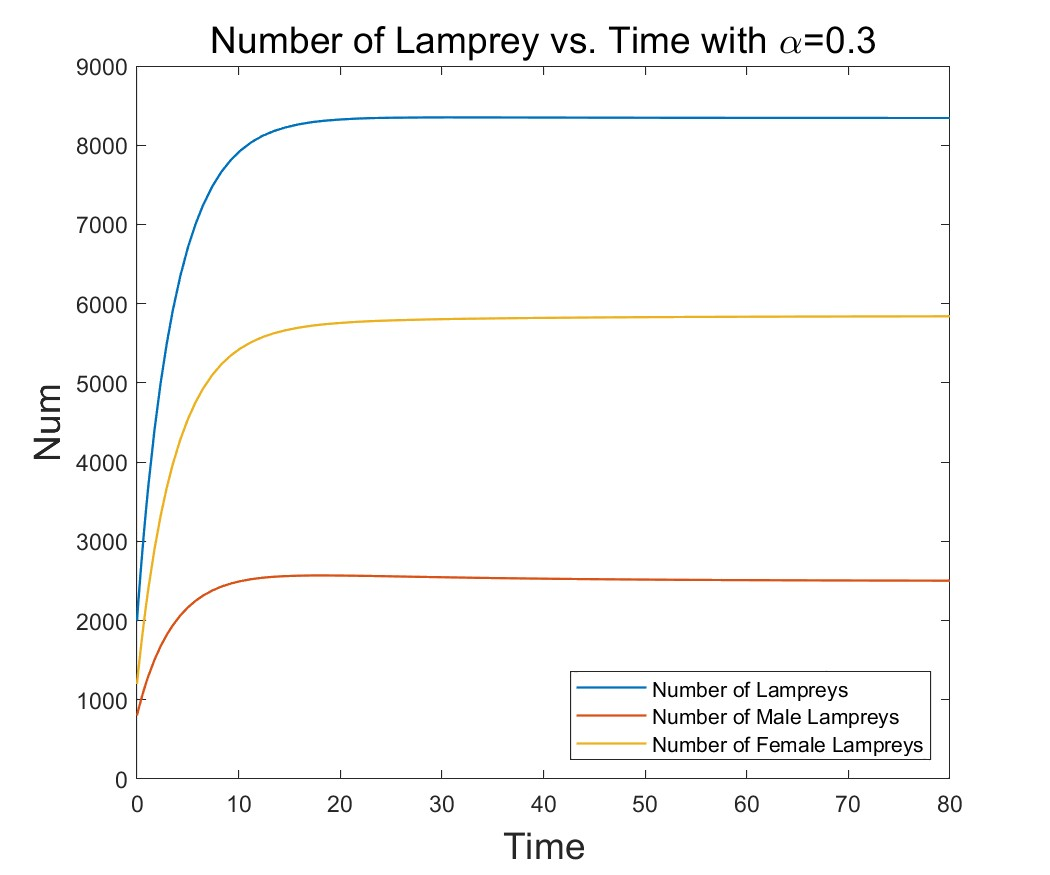
\includegraphics[width=0.3\textwidth]{alpha30.jpg}\label{alpha30}}
	\quad    % 重点就在这,优先横向排列,自动换行
	\subfloat[]
	{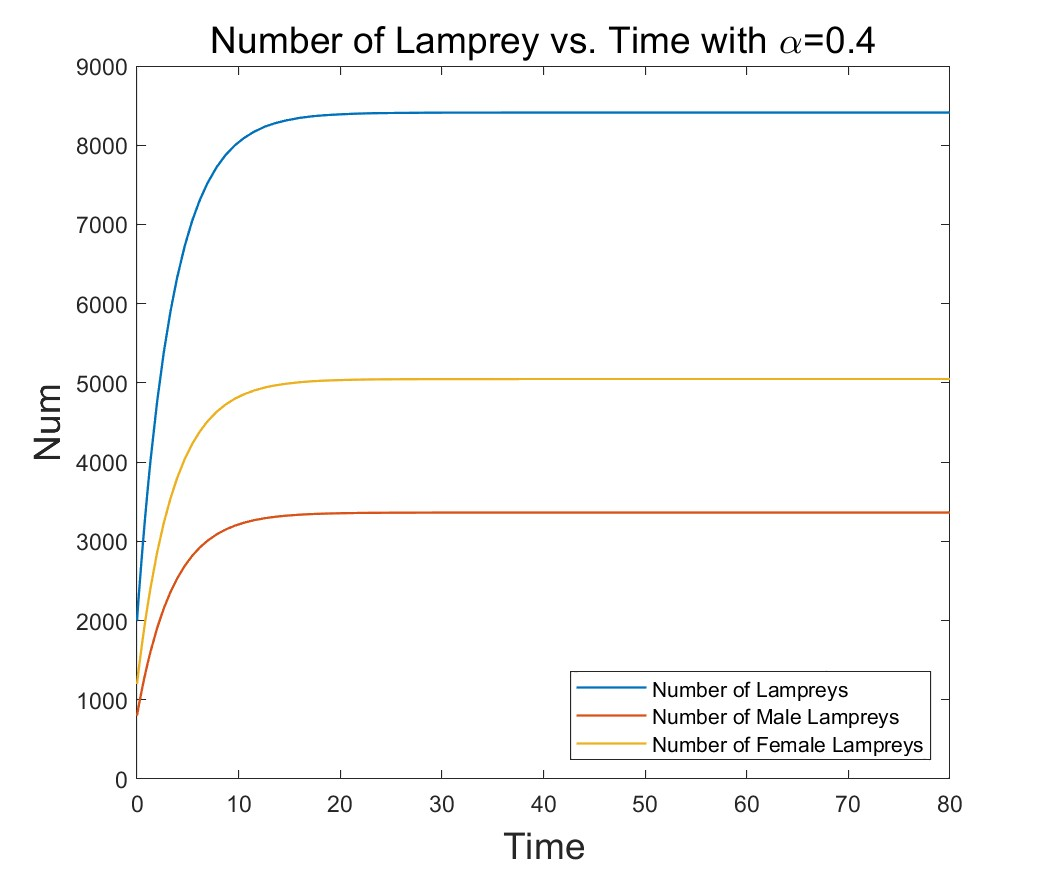
\includegraphics[width=0.3\textwidth]{alpha40.jpg}\label{alpha40}}
	\quad
	\subfloat[]
	{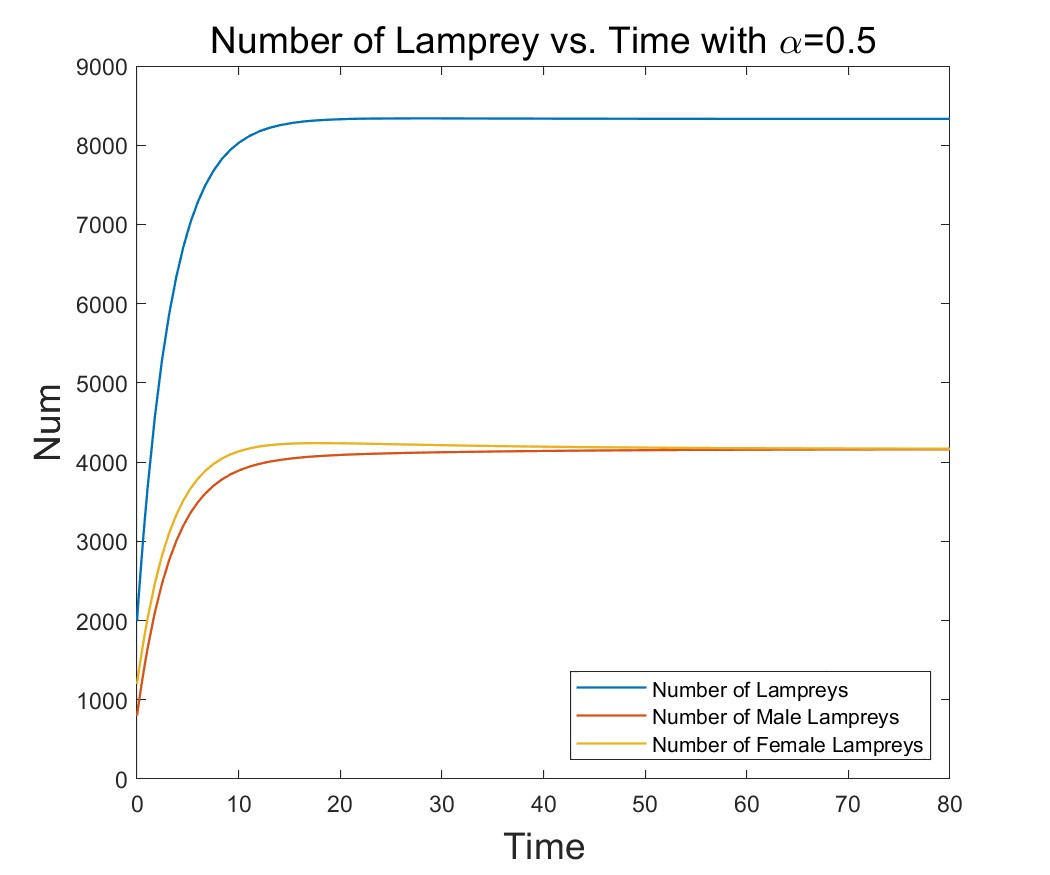
\includegraphics[width=0.3\textwidth]{alpha50.jpg}\label{alpha50}}
	\quad
	\subfloat[]
	{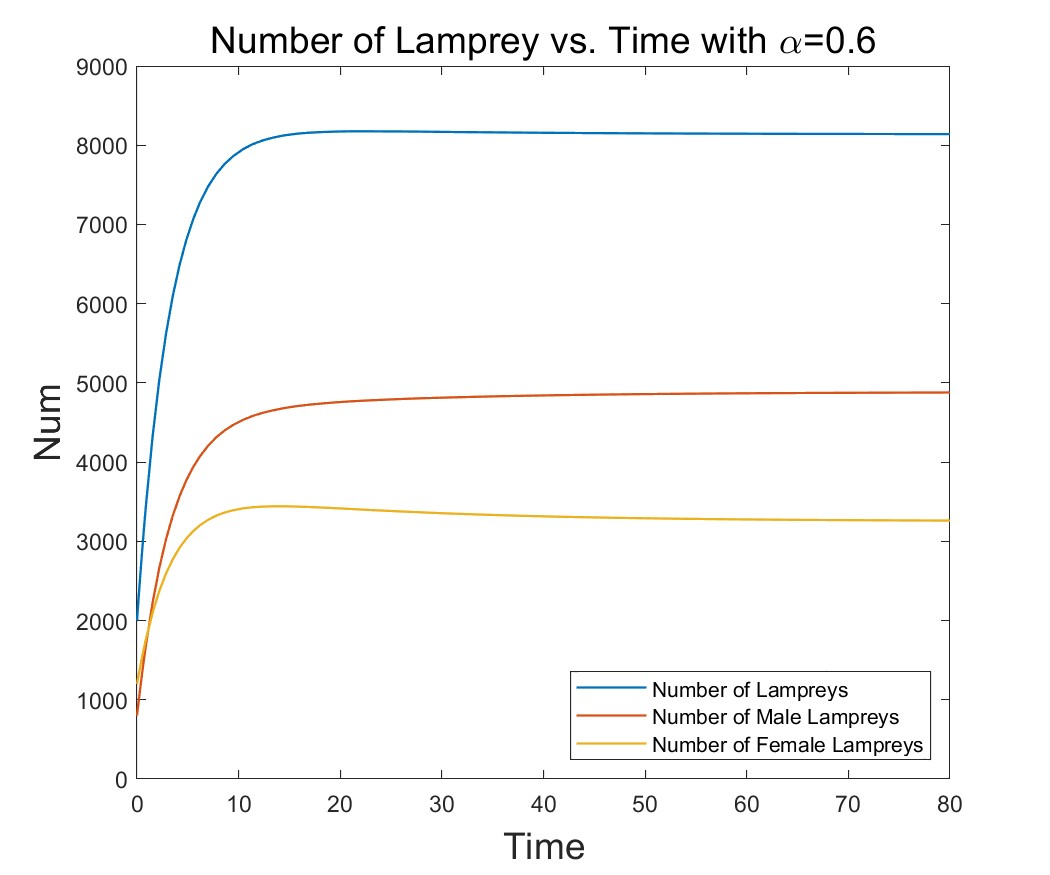
\includegraphics[width=0.3\textwidth]{alpha60.jpg}\label{alpha60}}
	\quad
	\subfloat[]
	{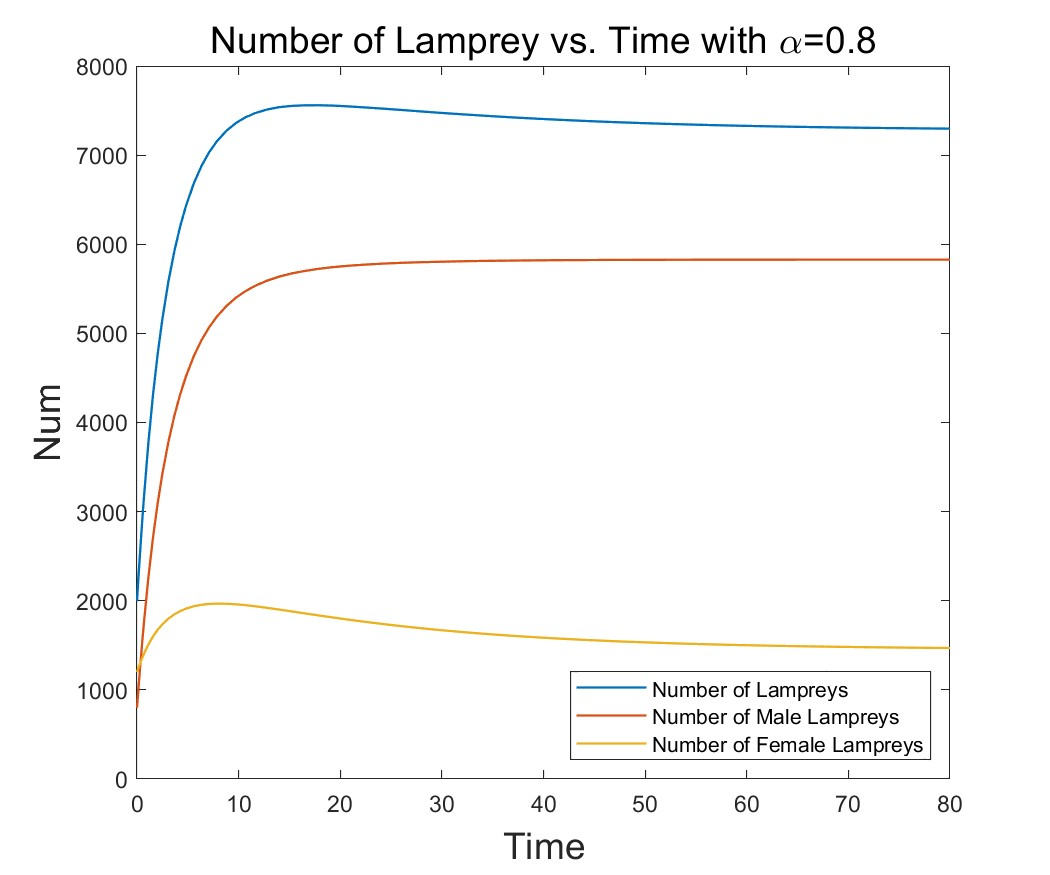
\includegraphics[width=0.3\textwidth]{alpha80.jpg}\label{alpha80}}
	\quad
	\subfloat[]
	{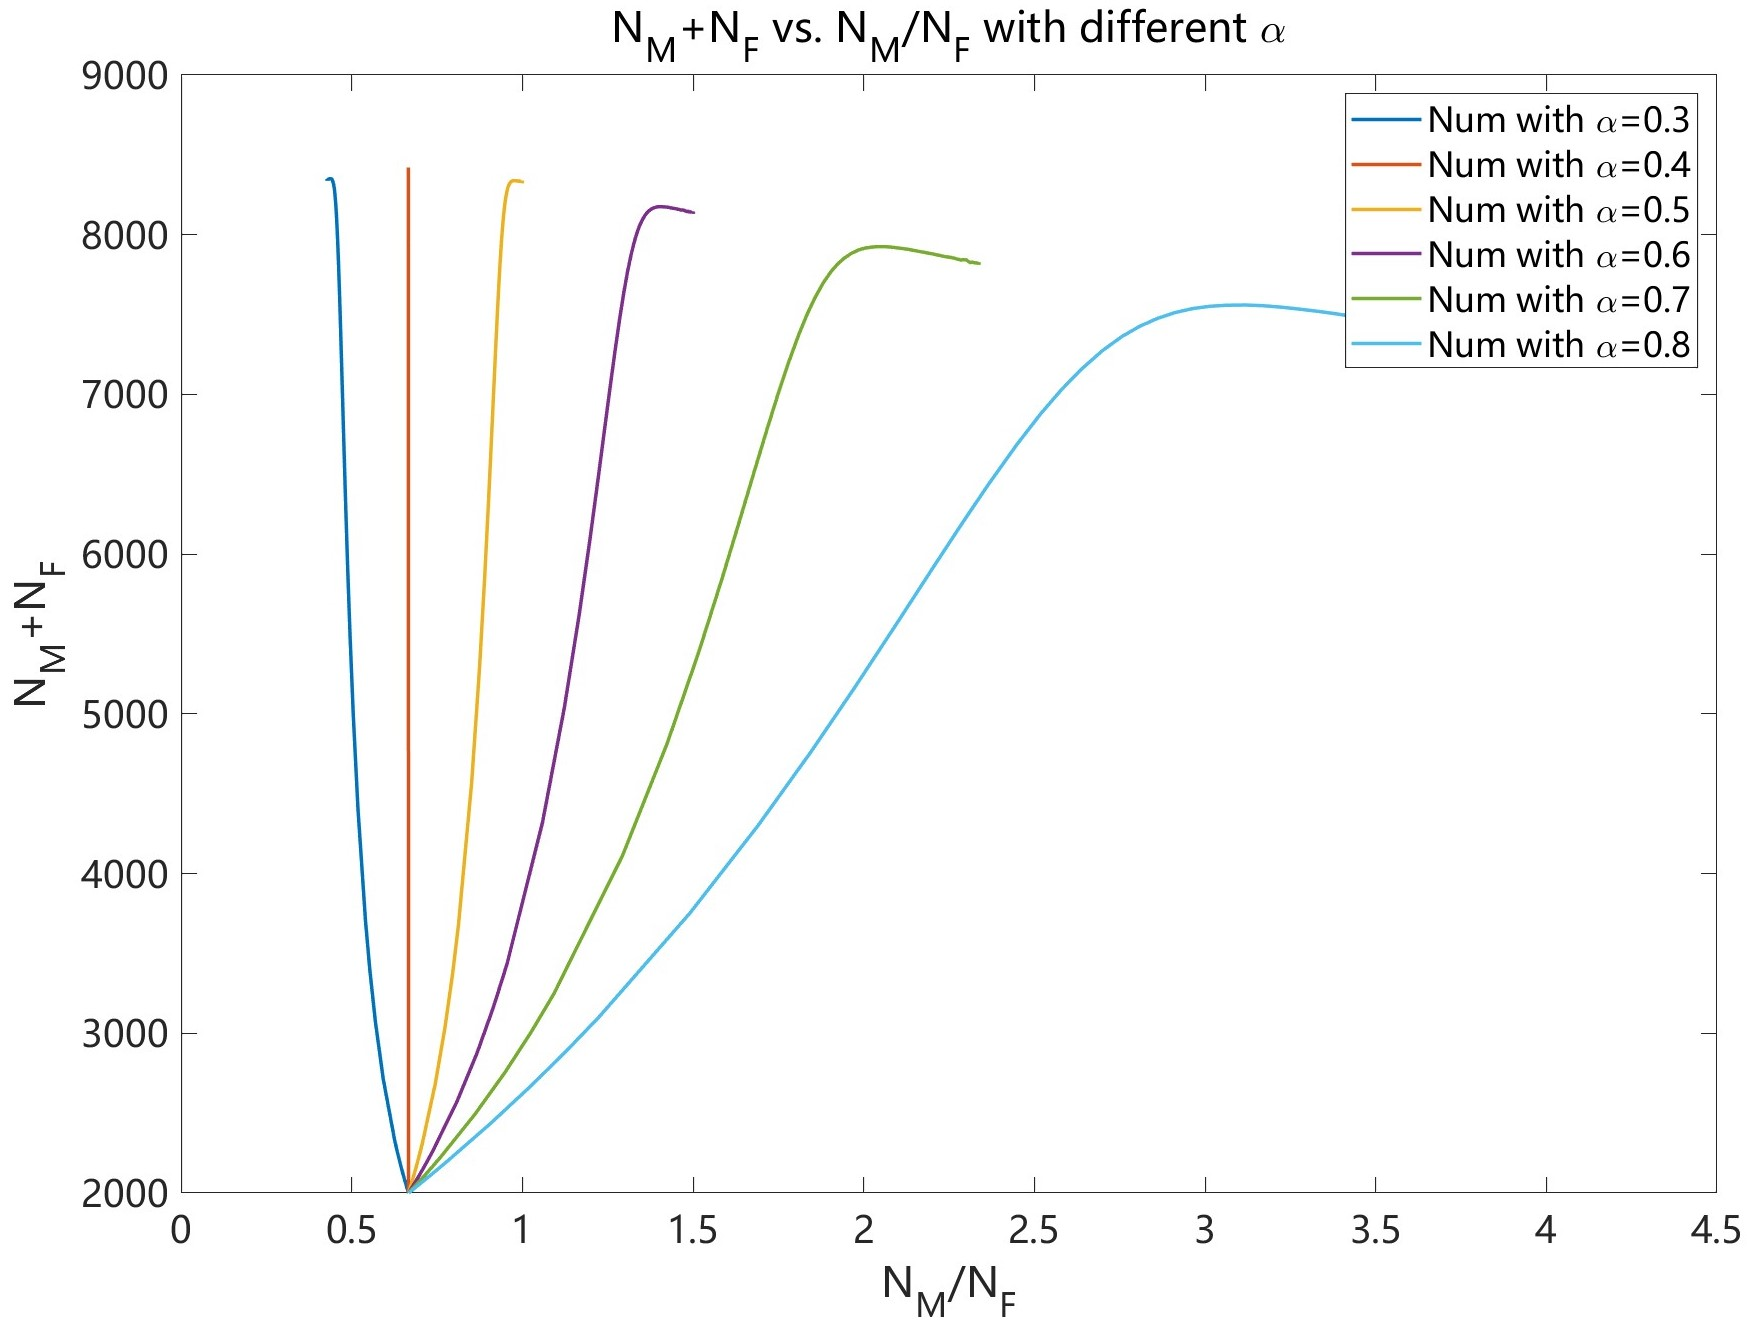
\includegraphics[width=0.3\textwidth]{M1-Num-ratio.jpg}\label{M1-Num-ratio}}
	\quad
	\caption{Num-sex ratio} \label{fig:3}
\end{figure}

In order to better study the impact of variable lamprey sex ratios on the environment, we use Figure \ref{fig:3} as a basis for integrating the curves into Figure \ref{subfig:left}. We find that the relationship between $RA$ and $alpha$ is not monotonic in the steady state, so we plot Figure \ref{subfig:right} to observe the relationship.

\begin{figure}[htbp]
	\centering
	\begin{subfigure}[b]{.45\textwidth}
		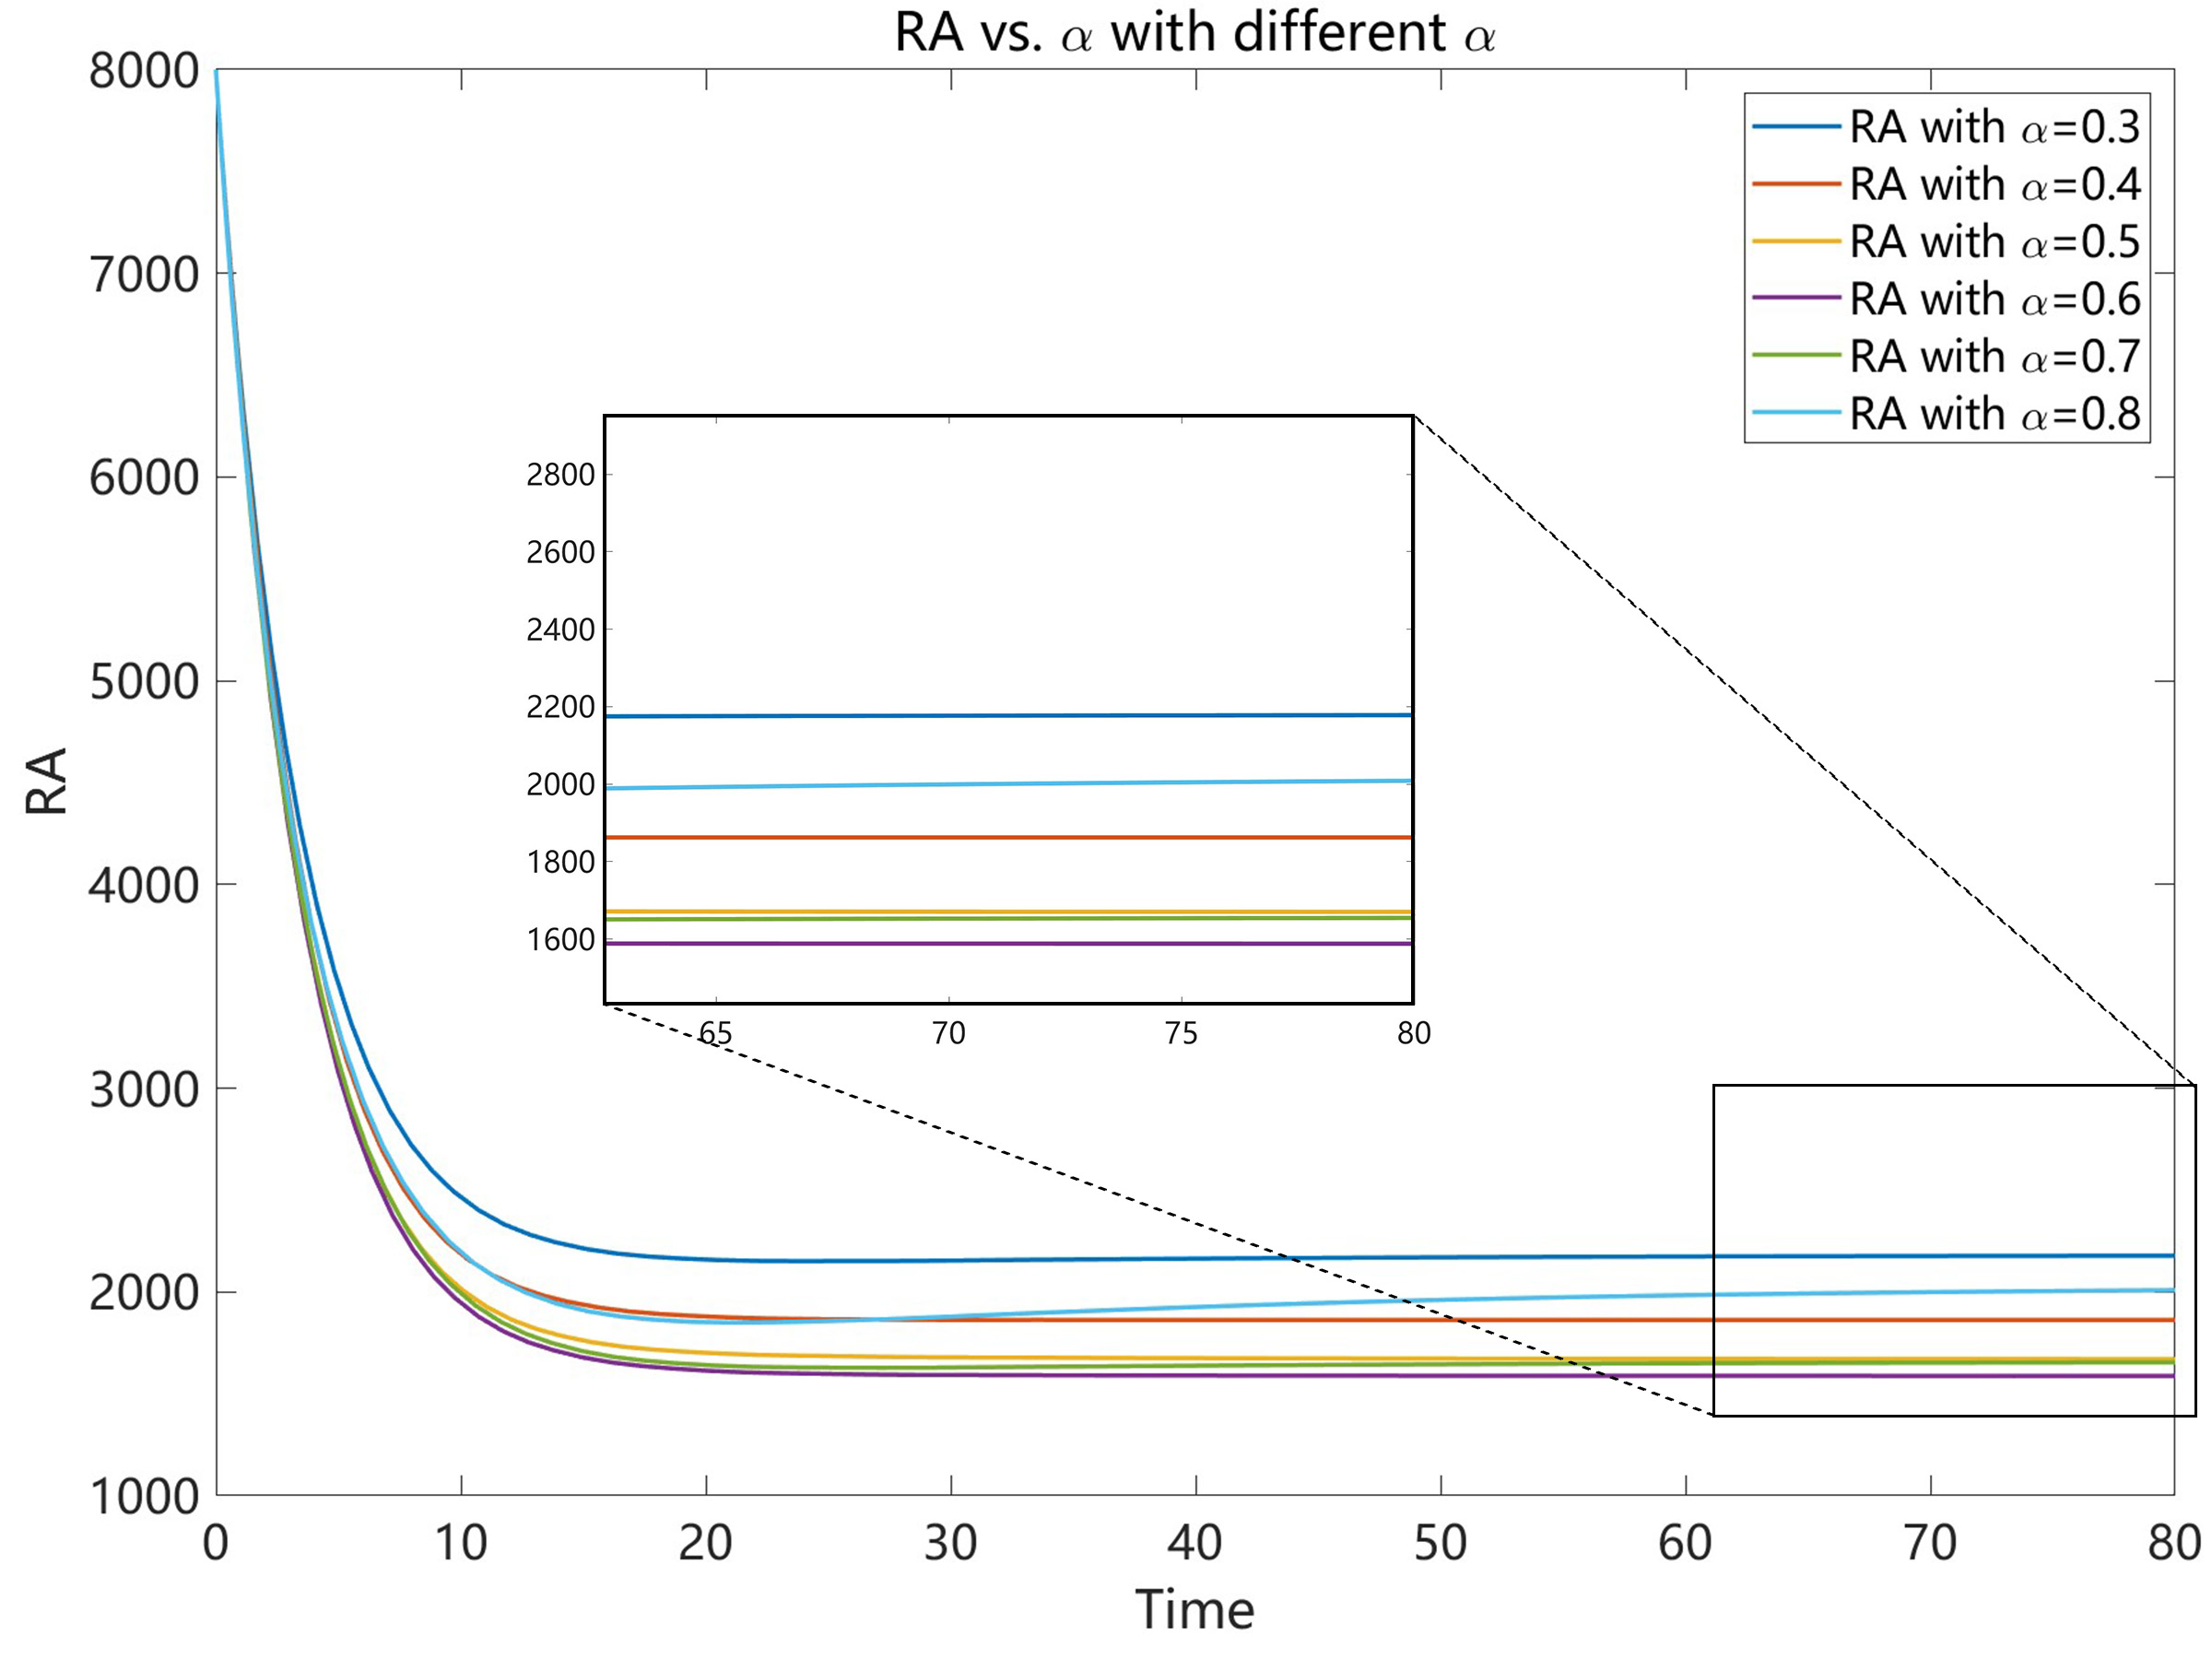
\includegraphics[width=\textwidth]{RA-TimeBig.jpg}
		\caption{\centering The variation of RA over time under different $\alpha$ conditions}\label{subfig:left}
	\end{subfigure}
	\begin{subfigure}[b]{.5\textwidth}
		\includegraphics[width=\textwidth]{RA-alpha.jpg}
		\caption{\centering The variation of RA over $\alpha$}\label{subfig:right}
	\end{subfigure}
	\caption{}\label{fig:subfigures}
\end{figure}

From Figure \ref{fig:subfigures}, there is corroboration between the two, as populations are more likely to reproduce under conditions of abundant resources, while there is little intraspecific competition, the population as a whole will show a tendency to take up more resources, making $alpha$ smaller, which is corroborated by the fact that in environments where food is more readily available, the proportion of males is less than 78\% of the population at around 56\%. Moreover, the $alpha$ value of 60\% corresponding to the very small value points in Figure \ref{subfig:right} obtained by the model is extremely close to 56\% of the real situation, indicating that the model works well.

To better reflect gender ratios and resource-hogging capacity, we use a heat map to visualize the consumption of resources by the lamprey population for different sex ratios; the lighter the color, the fewer the available resources, and the greater the impact of the lamprey on the ecosystem, reflecting the overall consumption of the population. The horizontal axis of the heat map is time, which is used to show the impact of population reproduction on the ecosystem at different times, and the vertical axis is the sex ratio, which is used to compare the different effects on environmental resources under different sex ratios.

Let's assume the same total number of resources available at the beginning, 80, and highlighting the squares when the initial resources drop to half, i.e. around 40, we can see that there is roughly a trend of convexity from the bottom right corner, i.e., the proportion of females rises and more resources are taken up as we follow the diagonal diagonal line downwards, which suggests that as the proportion of females in the population becomes larger, the population as a whole has a greater ability to consume the resources it does consume. And the more material and energy that is available in a population, the more favorable it is for the development of the population itself, allowing for greater resources in the ecosystem to be consumed quickly.
\clearpage
Ultimately, from Figure \ref{M1-Num-ratio}, we conclude that when sex ratios can be varied, the proportion of females rises in the face of ample resources, allowing the population to reproduce faster and take up more resources.This is the impact on the larger ecological system when the population of lampreys can alter its sex ratio.

\begin{figure}[htbp]
	\centering
	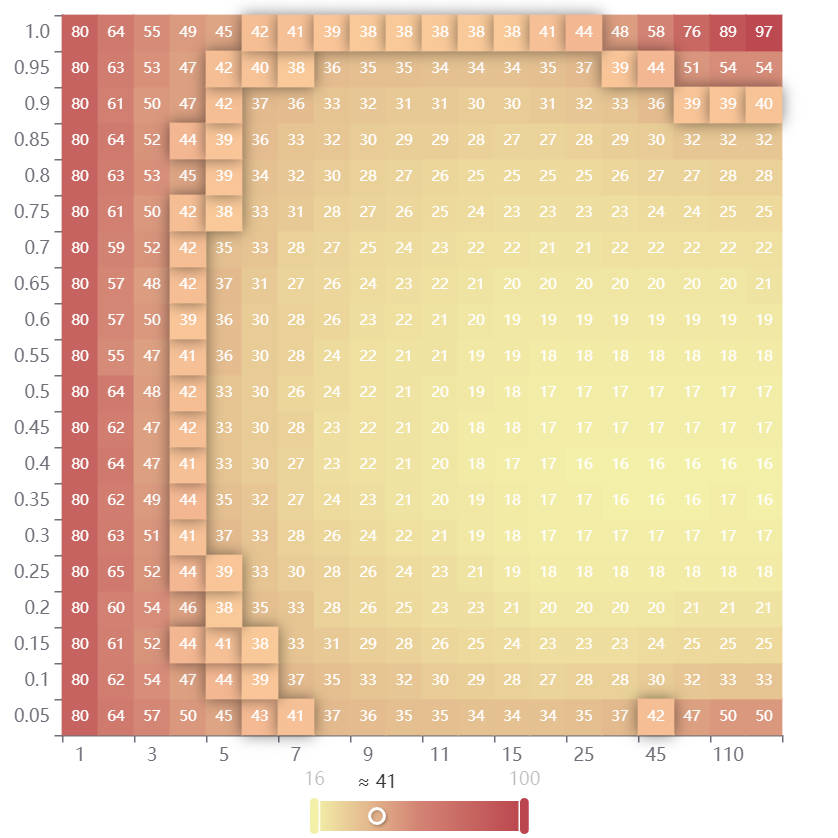
\includegraphics[width=.6\textwidth]{red pic.jpg}
	\caption{Heat map of resource availability}\label{red}
\end{figure}



\section{Model 2: Sex Ratio Resource Consumption with Prey Model}
\subsection{Description of a Predator-prey Chain}
Since in the real situation, combined with the model of Model 1, we can know that as the population occupies more resources, the number $TNL$ becomes more, the resources allocated to each individual will decrease, which will lead to a slower growth rate of the individuals in the population, and because it is known that when the growth rate is lower, the larvae follow the tendency to differentiate into males, so the resource availability leads to the change of the sex ratio, and also due to the sex ratio will also influence the lamprey population's and because sex ratio also affects the predatory capacity (resource occupancy) of lamprey populations, which in turn affects resource availability\cite{8}. 

Therefore, when lamprey populations are introduced into an ecosystem and the interactions between different populations are considered, there is bound to be a feedback relationship in this, leading to a dynamic change in the sex ratio. Therefore, in this model, we consider the dynamic change in sex ratio and write its dynamical equation related to the change in available resources, while introducing a predator model to investigate the advantages and disadvantages of this change by exploring how sex ratio affects lamprey predation.

According to the conditions given in the question, $\alpha$ is around 56\% in the nutrient sufficient case and 78\% in the nutrient-poor case, then we introduce the min-max standardized formula for optimization, assuming that the nutrient layers are uniformly distributed, and each layer corresponds to a male conversion rate of lampreys ranging from
56\% to 78\%, and thus derive equation:

\begin{equation}\label{eq:5-1}
	\alpha = 56\% + \frac{78\%-56\%}{{RA}_{max}-0}({RA}_{max}-RA)
\end{equation}

References to models in Model 1 (\ref{eq:4-8}) (\ref{eq:4-11}):
\begin{equation}\label{eq:5-2}
\begin{cases}
	\frac{\mathrm{d}N_{M}}{\mathrm{d}t}=r \cdot \alpha RA-\beta N_{M} - \frac{rRA}{\lambda}\\ \\
	\frac{\mathrm{d}N_{F}}{\mathrm{d}t}=r \cdot(1 - \alpha )RA-\beta N_{F} - \frac{rRA}{\lambda} \\ \\
	r = c\frac{N_{F}N_{M}}{(TNL)^{2}}
\end{cases}
\end{equation}
However, given the different metrics we refer to, we treat $rRA$ in Model 1. It is a measure of the reproduction rate of lamprey, and we know by analogy from the Lotka–Volterra equation that $rRA$ is proportional to the number of trapped organisms, denoted as $U$.

$rRA$ is directly proportional to the ability and number of male and female lampreys to feed, so we can set out the relationship:
\begin{equation}\label{eq:5-3}
rRA = \epsilon_{1} U (a_{F}N_{F}+a_{M}N_{M})
\end{equation}
where $\epsilon_1$ is the predator-to-prey predation conversion factor for predators

Based on the Lotka-Volterra equation corrected for the different predation abilities of male and female lampreys, we can obtain an equation for the rate of change of the prey:

\begin{equation}\label{eq:5-4}
\frac{\mathrm{d}U}{\mathrm{d}t}=hU-\epsilon_{2}U(a_{F}N_{F}+a_{M}N_{M})
\end{equation}

where $h$ is the natural growth rate of the prey and $\epsilon_2$ is the prey-to-predator predation conversion coefficient, combining the above equations and relationships we can conclude that:

\begin{equation}\label{eq:5-5}
\begin{cases}
	\frac{\mathrm{d}N_{M}}{\mathrm{d}t}=\left( \alpha-\frac{1}{\lambda} \right)\epsilon_{1}U(a_{F}N_{F}+a_{M}N_{M}) - \beta N_M\\ \\

	\frac{\mathrm{d}N_{F}}{\mathrm{d}t}=\left( 1- \alpha-\frac{1}{\lambda} \right)\epsilon_{1}U(a_{F}N_{F}+a_{M}N_{M}) - \beta N_F\\ \\
	\frac{\mathrm{d}U}{\mathrm{d}t}=hU-\epsilon_{2}U(a_{F}N_{F}+a_{M}N_{M})
\end{cases}
\end{equation}
Using Matlab for solving model, we can get the relationship between lampreys and prey.

\subsection{Analysis of the Result}
From Figure \ref{M2-Num-Time-ExtLong}, we can see that when the sex ratio is variable, although the total number of individuals in the population fluctuates normally due to inter-population interactions, it gradually stabilizes and converges to a value in the long run. From Figure \ref{M2-Num-Time-Long}, we can see that this convergence process is somewhat periodicity, so we choose one of the segments, as shown in Figure \ref{M2-Num-Time}, to analyze:

\begin{figure}[!h]
	\centering
	\subfloat[]
	{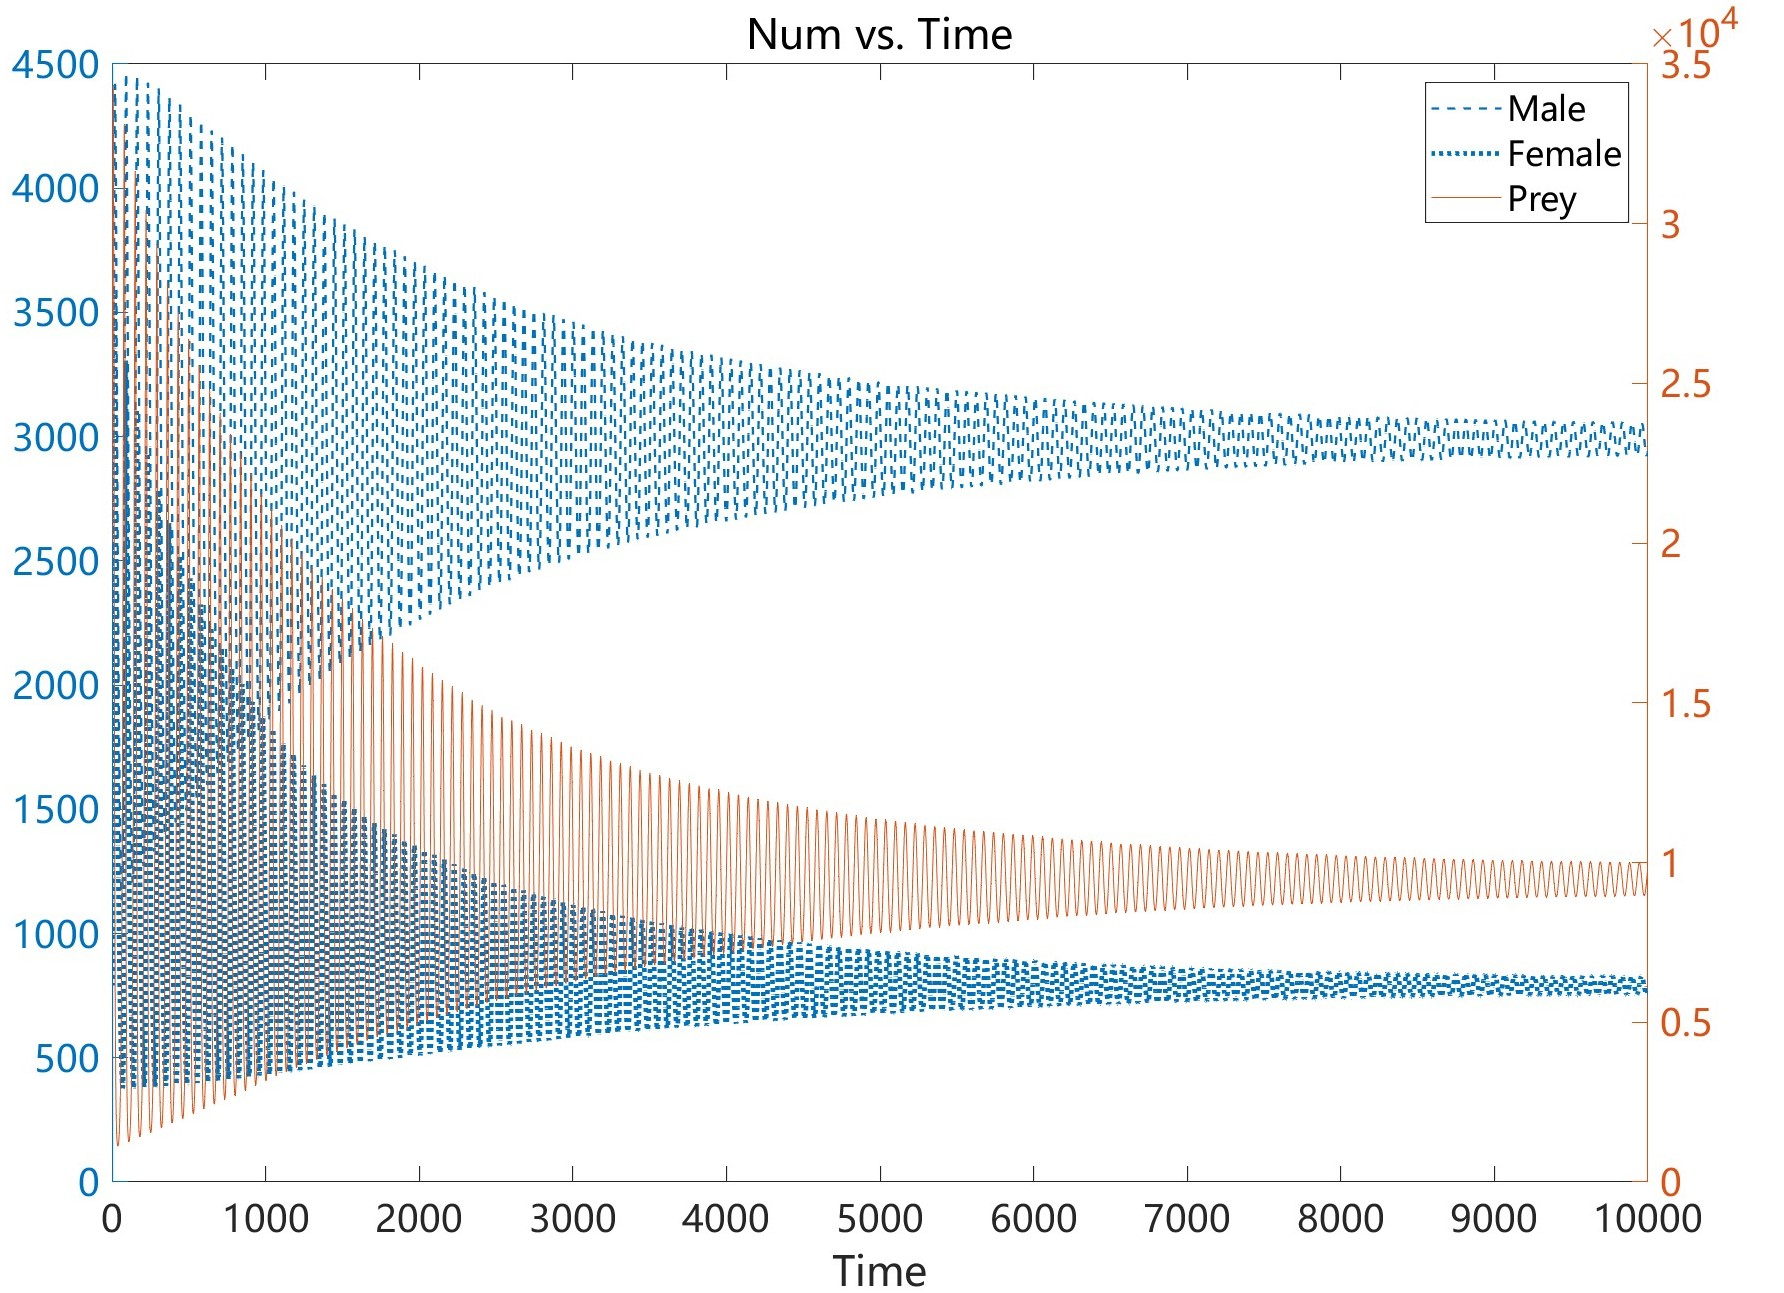
\includegraphics[width=0.3\textwidth]{M2-Num-Time-ExtLong.jpg}\label{M2-Num-Time-ExtLong}}
	\quad    % 重点就在这,优先横向排列,自动换行
	\subfloat[]
	{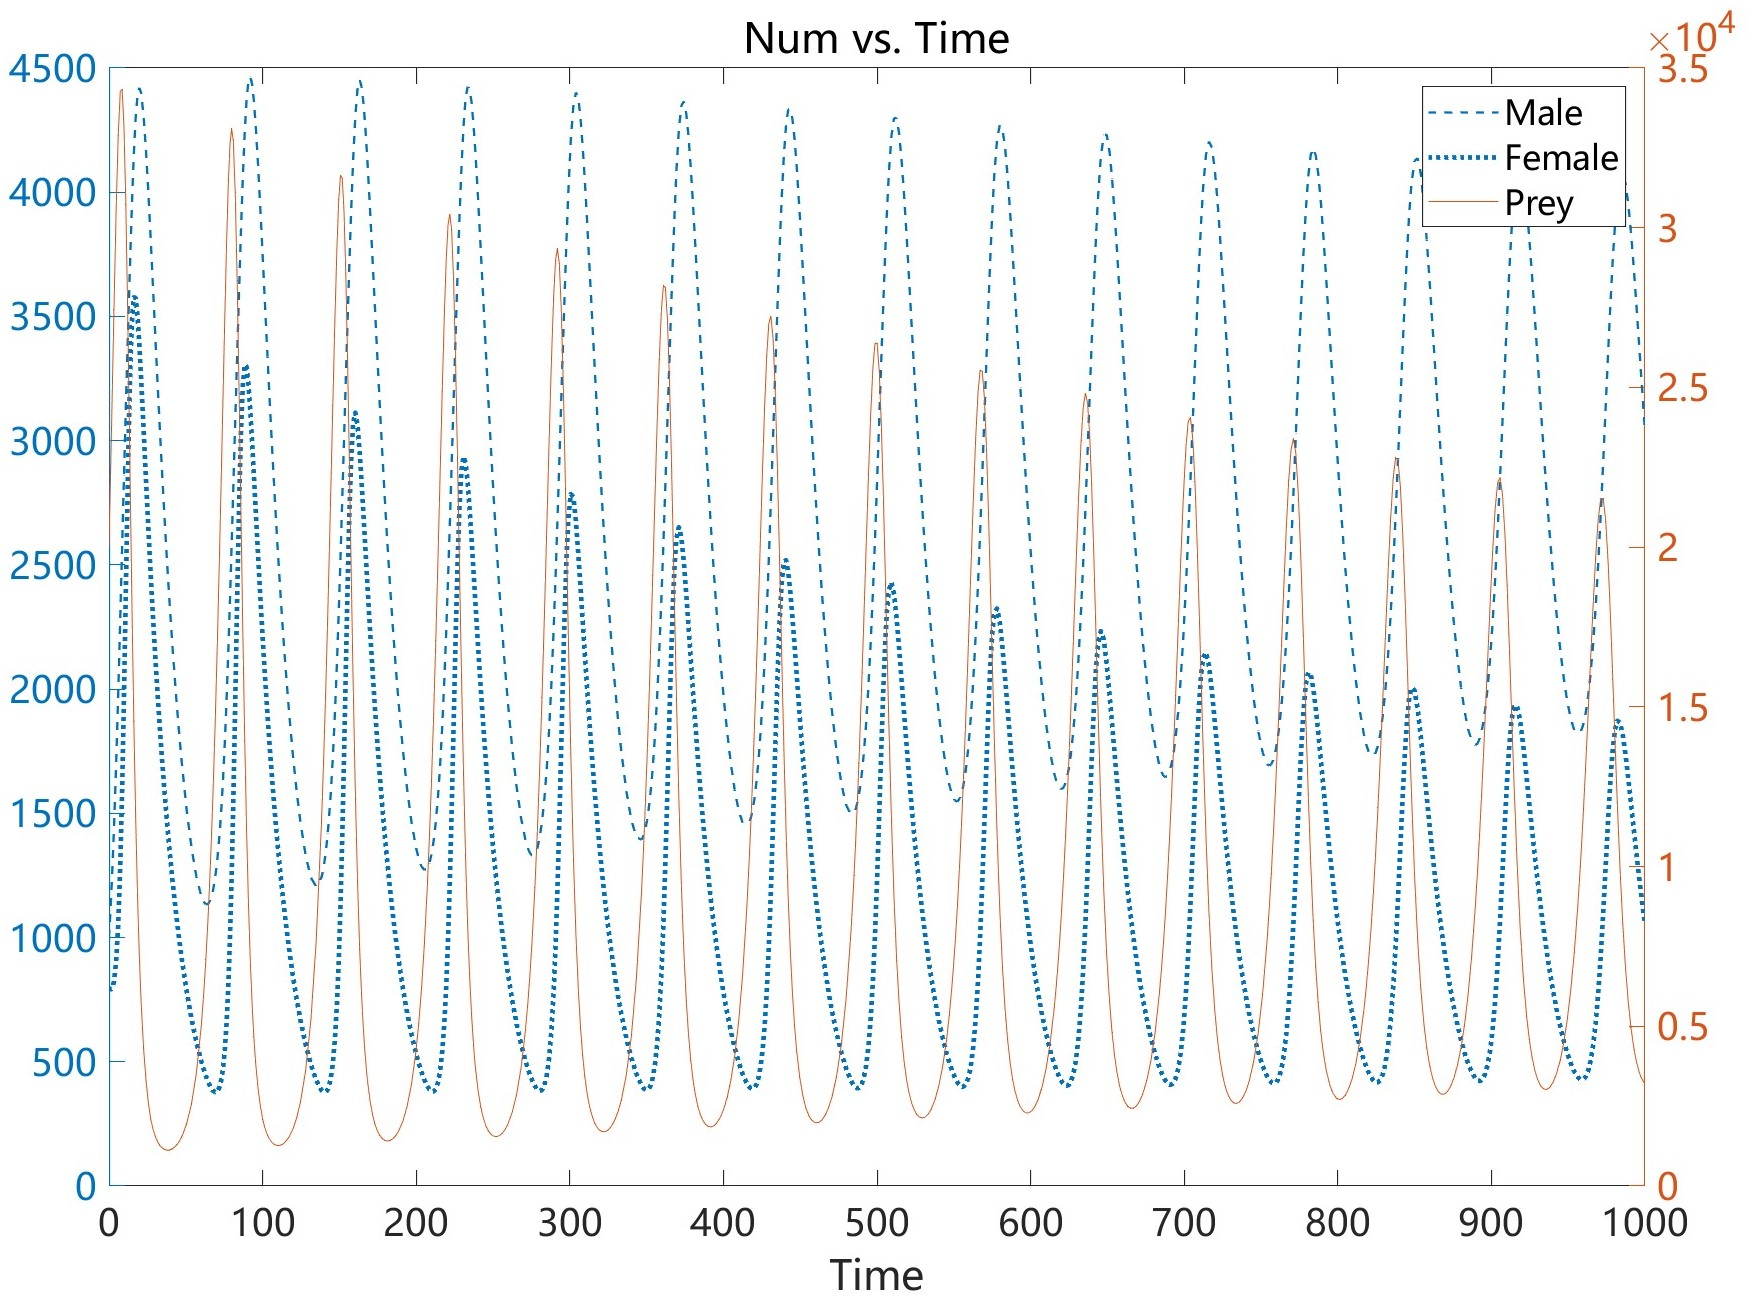
\includegraphics[width=0.3\textwidth]{M2-Num-Time-Long.jpg}\label{M2-Num-Time-Long}}
	\quad
	\subfloat[]
	{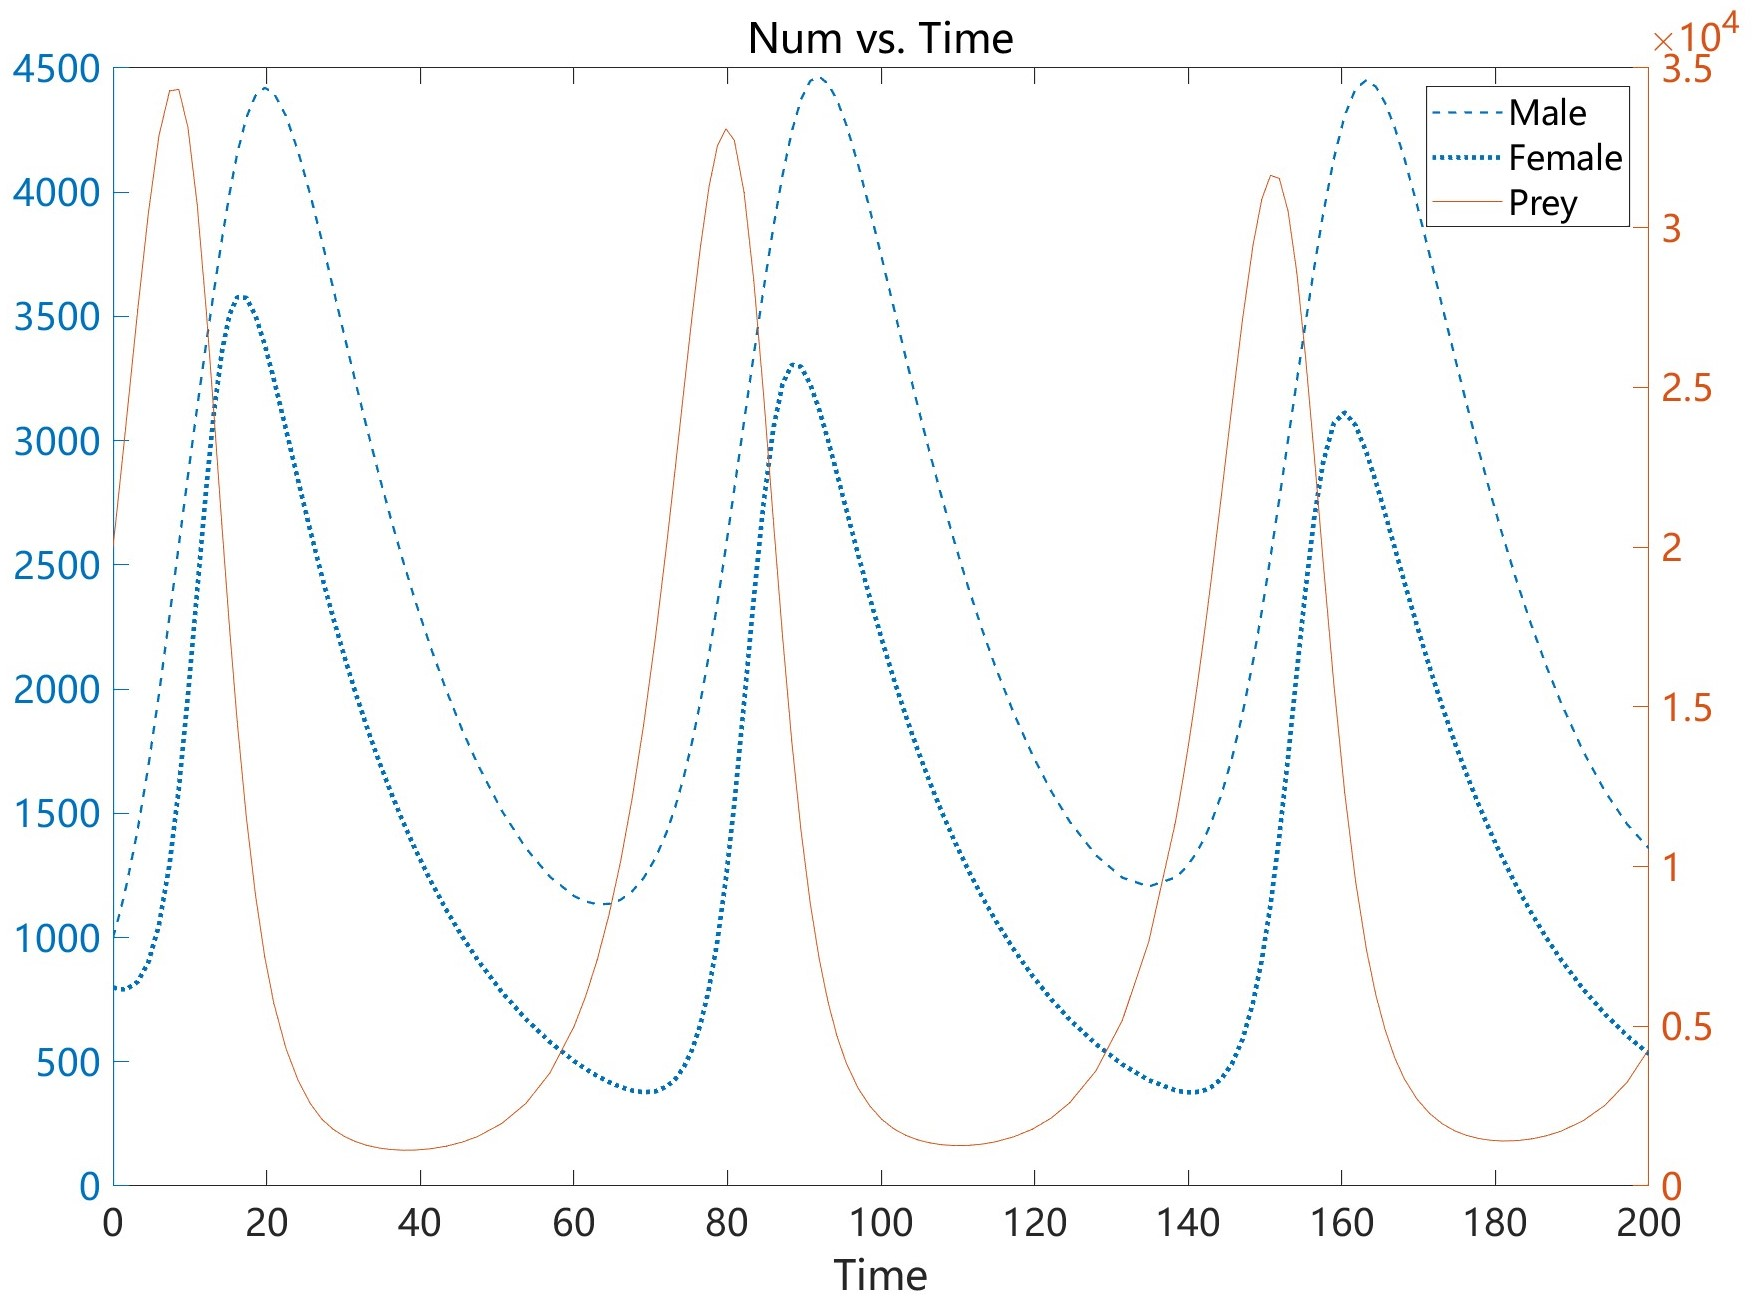
\includegraphics[width=0.3\textwidth]{M2-Num-Time.jpg}\label{M2-Num-Time}}
	\quad	
	\caption{Changes of populations in ecosystems}
\end{figure}

First, we can see that at the extreme point of the Prey curve, when the predators are the most numerous, i.e., when the RA is the largest, the sex ratio is close to 56\%, which is
in line with the actual situation, indicating that the model reflects the actual situation well.

Then, we can see that when there are fewer predators, $RA$ decreases and females decline faster, and it is known from the literature that males are longer, more adaptable to their environment, and are better able to survive and continue populations in harsh environments \cite{4}\cite{9}. So, when things decrease, the lamprey sex ratio changes so that males make up a larger percentage of the population, allowing females to decline more rapidly and allowing males to relatively increase and the population to adapt more.

Meanwhile, in conjunction with Model 1, it can be seen from Figure \ref{M1-Num-ratio} that when resources are sufficient, the population reproduces faster and ultimately in greater numbers if there are more females. What's more, from the Table \ref{L and W}, the male is stronger to cope with the pressure. So, this illustrates the advantage of variable sex ratios, which is the ability to increase the proportion of males when resources are low, enough to cope with environmental pressures. It can also lower the proportion of males when resources are high, increasing the rate at which the population reproduces.

\begin{table}[!htbp]
	\begin{center}
		\begin{threeparttable}
			\caption{The data of sea lamprey}
			\begin{tabular}{ccccc}
				\toprule
				\multicolumn{1}{m{4cm}}{\centering Tributary}
				&\multicolumn{1}{m{2cm}}{\centering The Length of Males(mm)}
				&\multicolumn{1}{m{2cm}}{\centering The Length of Males(mm)}
				&\multicolumn{1}{m{2cm}}{\centering The Weight of Males(g)}
				&\multicolumn{1}{m{3cm}}{\centering The Weight of Females(g)}\\
				\midrule
				$Tittabawassee R.(F)$&472&468&243&218\\
				$East Au Gres R.(G)$&490&470&242&245\\
				$Trout R. (J)$ &475&475&237&236\\
				$Cheboygan R.(M)$ &485&481&231&237\\
				$Albany Cr. (P)$ &477&469&226&216\\
				$St. Marys R.(A)$ &481&497&233&262\\
				
				\bottomrule
			\end{tabular}\label{L and W}
			\small
			\textit{* The data is from Great Lakes Fishery Commission \cite{6}}
		\end{threeparttable}
	\end{center}
\end{table}
And, we use the number of lampreys and their predators as the axes of a Cartesian coordinate system to create a phase diagram, to make lamprey-prey interactions more visible and preparing for subsequent quantification.

As can be seen, Figure \ref{subfig:M2-Lamprey-Prey} represents the relationship between the two population changes as time tends to infinity, when the number of prey begins to rise, followed shortly thereafter by the number of lampreys. As there is more prey to catch, the $RA$ becomes larger and the growth rate becomes larger. After the lamprey population increases, over-hunting causes the population size of the prey to decrease. As a result, the prey on which it depends for its own survival decreases, $RA$ decreases, and the number of lampreys decreases. At this point, because the threat from lampreys is reduced, the prey population begins to reproduce faster again and the population size climbs rapidly. And so on and so forth. The fluctuation of the predator population always shows a lag effect of about a quarter of a cycle compared to the prey population, and we can visualize the relationship between the prey and predator population sizes.

In Figure \ref{subfig:M2-Lamprey-Prey-ChangeableAlpha}, we fixed the sex differentiation ratio of juvenile lamprey, and we can find that the magnitude of the curve is significantly larger, and the area of the curve is much larger than the area corresponding to the variable sex ratio, which indicates that the stability of the lamprey population becomes worse when the sex ratio is fixed, and illustrates the advantage of the variable sex ratio - making the lamprey population more stable.
\begin{figure}[htbp]
	\centering
	\begin{subfigure}[b]{.45\textwidth}
		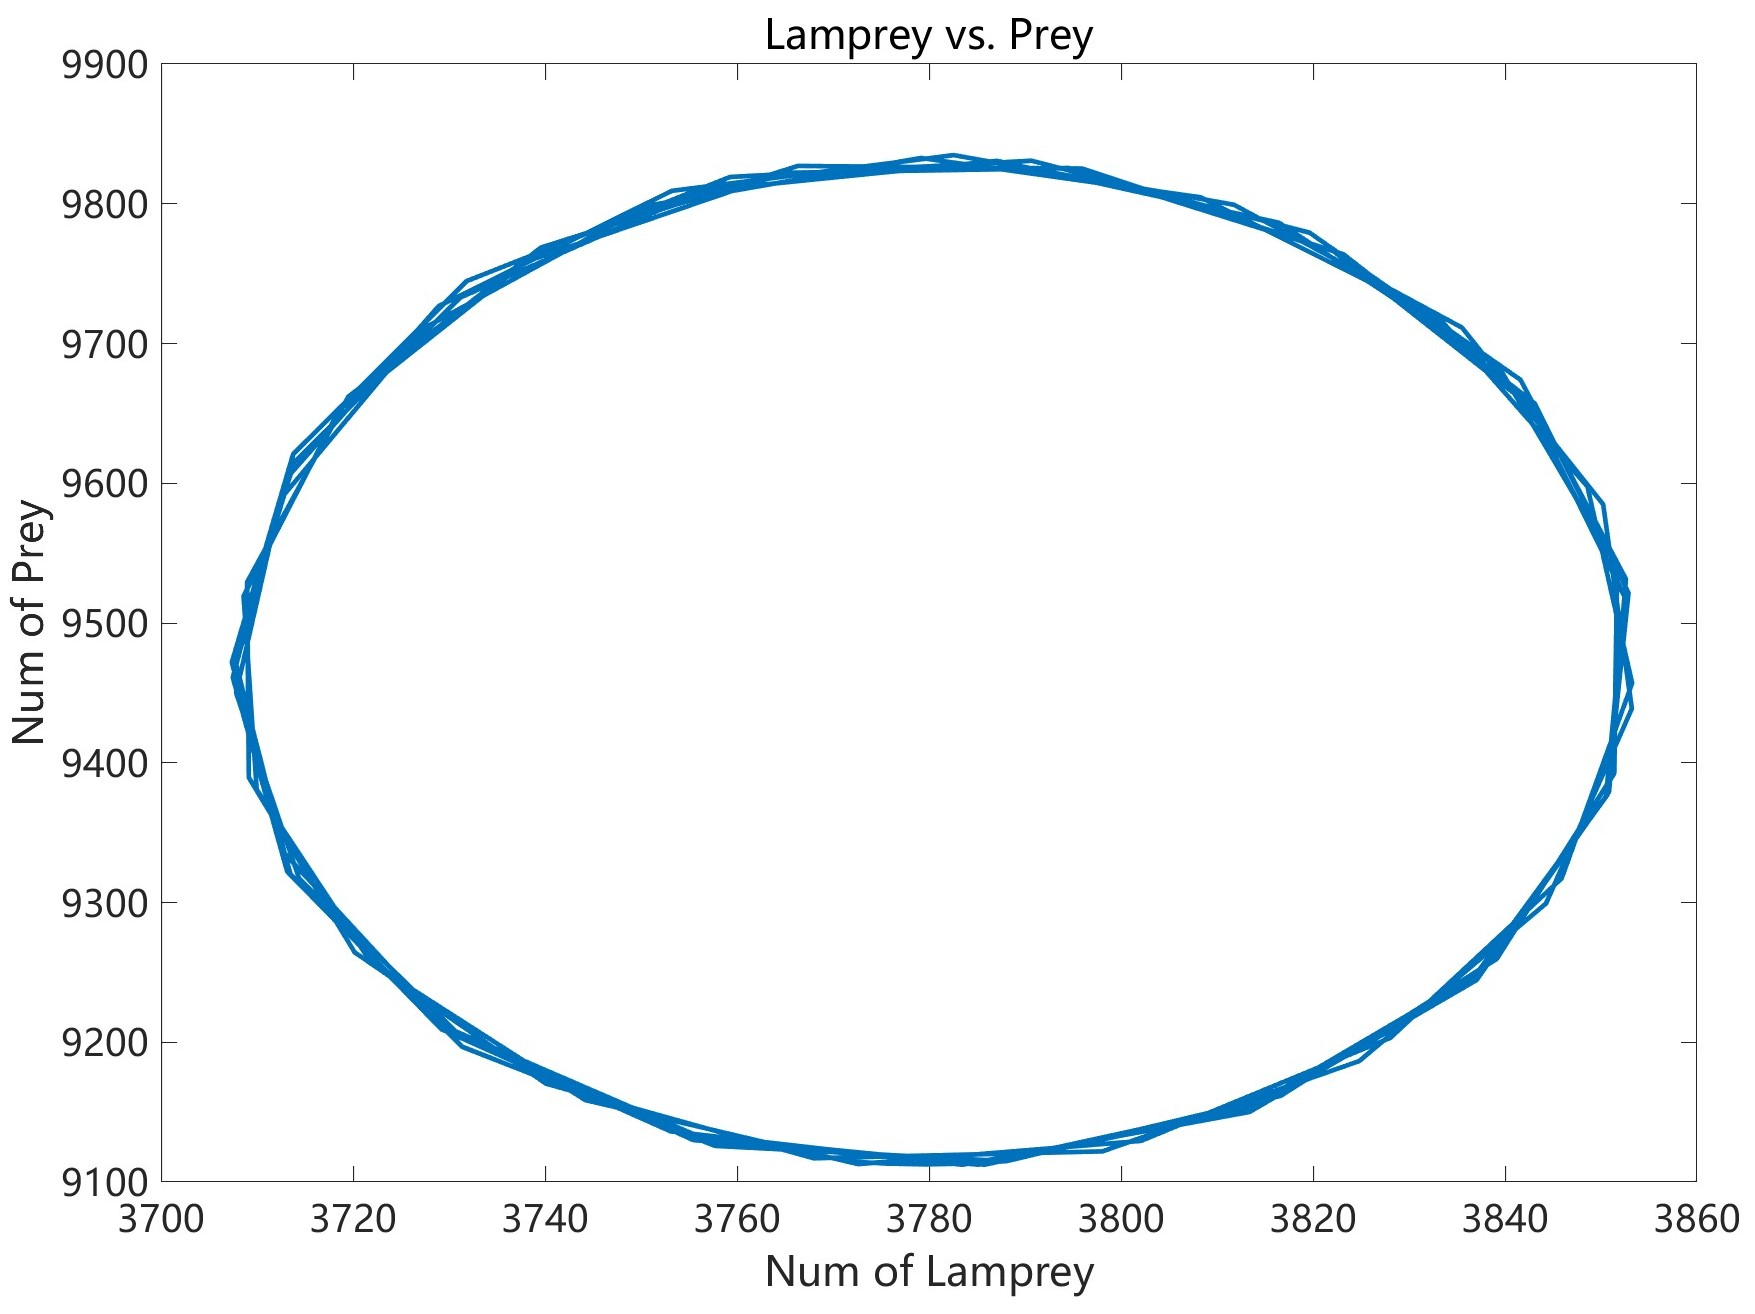
\includegraphics[width=\textwidth]{M2-Lamprey-Prey.jpg}
		\caption{$\alpha$ is changeable}\label{subfig:M2-Lamprey-Prey}
	\end{subfigure}
	\begin{subfigure}[b]{.45\textwidth}
		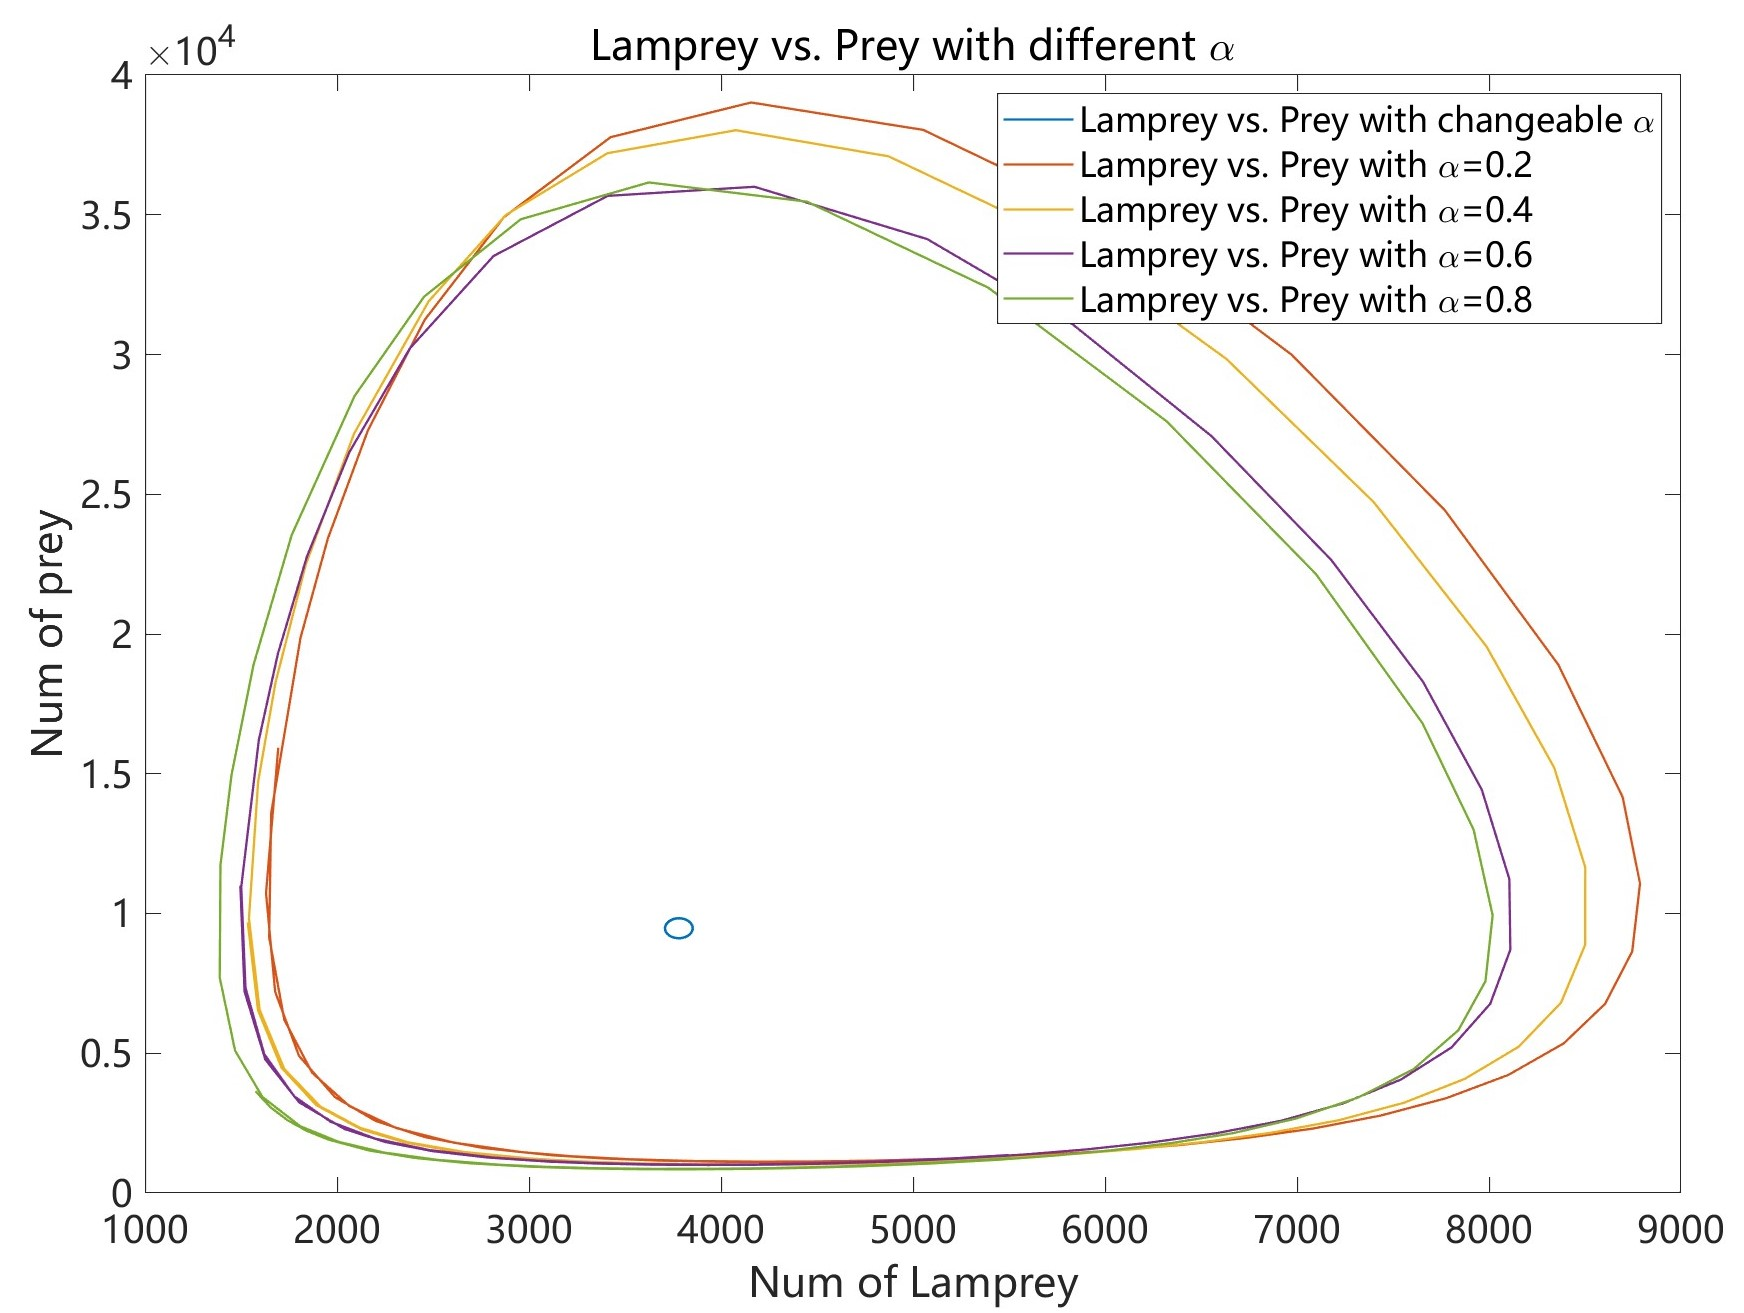
\includegraphics[width=\textwidth]{M2-Lamprey-Prey-ChangeableAlpha.jpg}
		\caption{$\alpha$ is fixed}\label{subfig:M2-Lamprey-Prey-ChangeableAlpha}
	\end{subfigure}
	\caption{phase trajectory diagram}\label{fig:07}
\end{figure}

However, this also has the disadvantage that when the male to female ratio deviates too far from 1:1, the risk of extinction on one side increases, and in populations that can only reproduce sexually, the extinction of one sex means the extinction of the population \cite{11}.
\begin{figure}[htbp]
	\centering
	\begin{subfigure}[b]{.6\textwidth}
		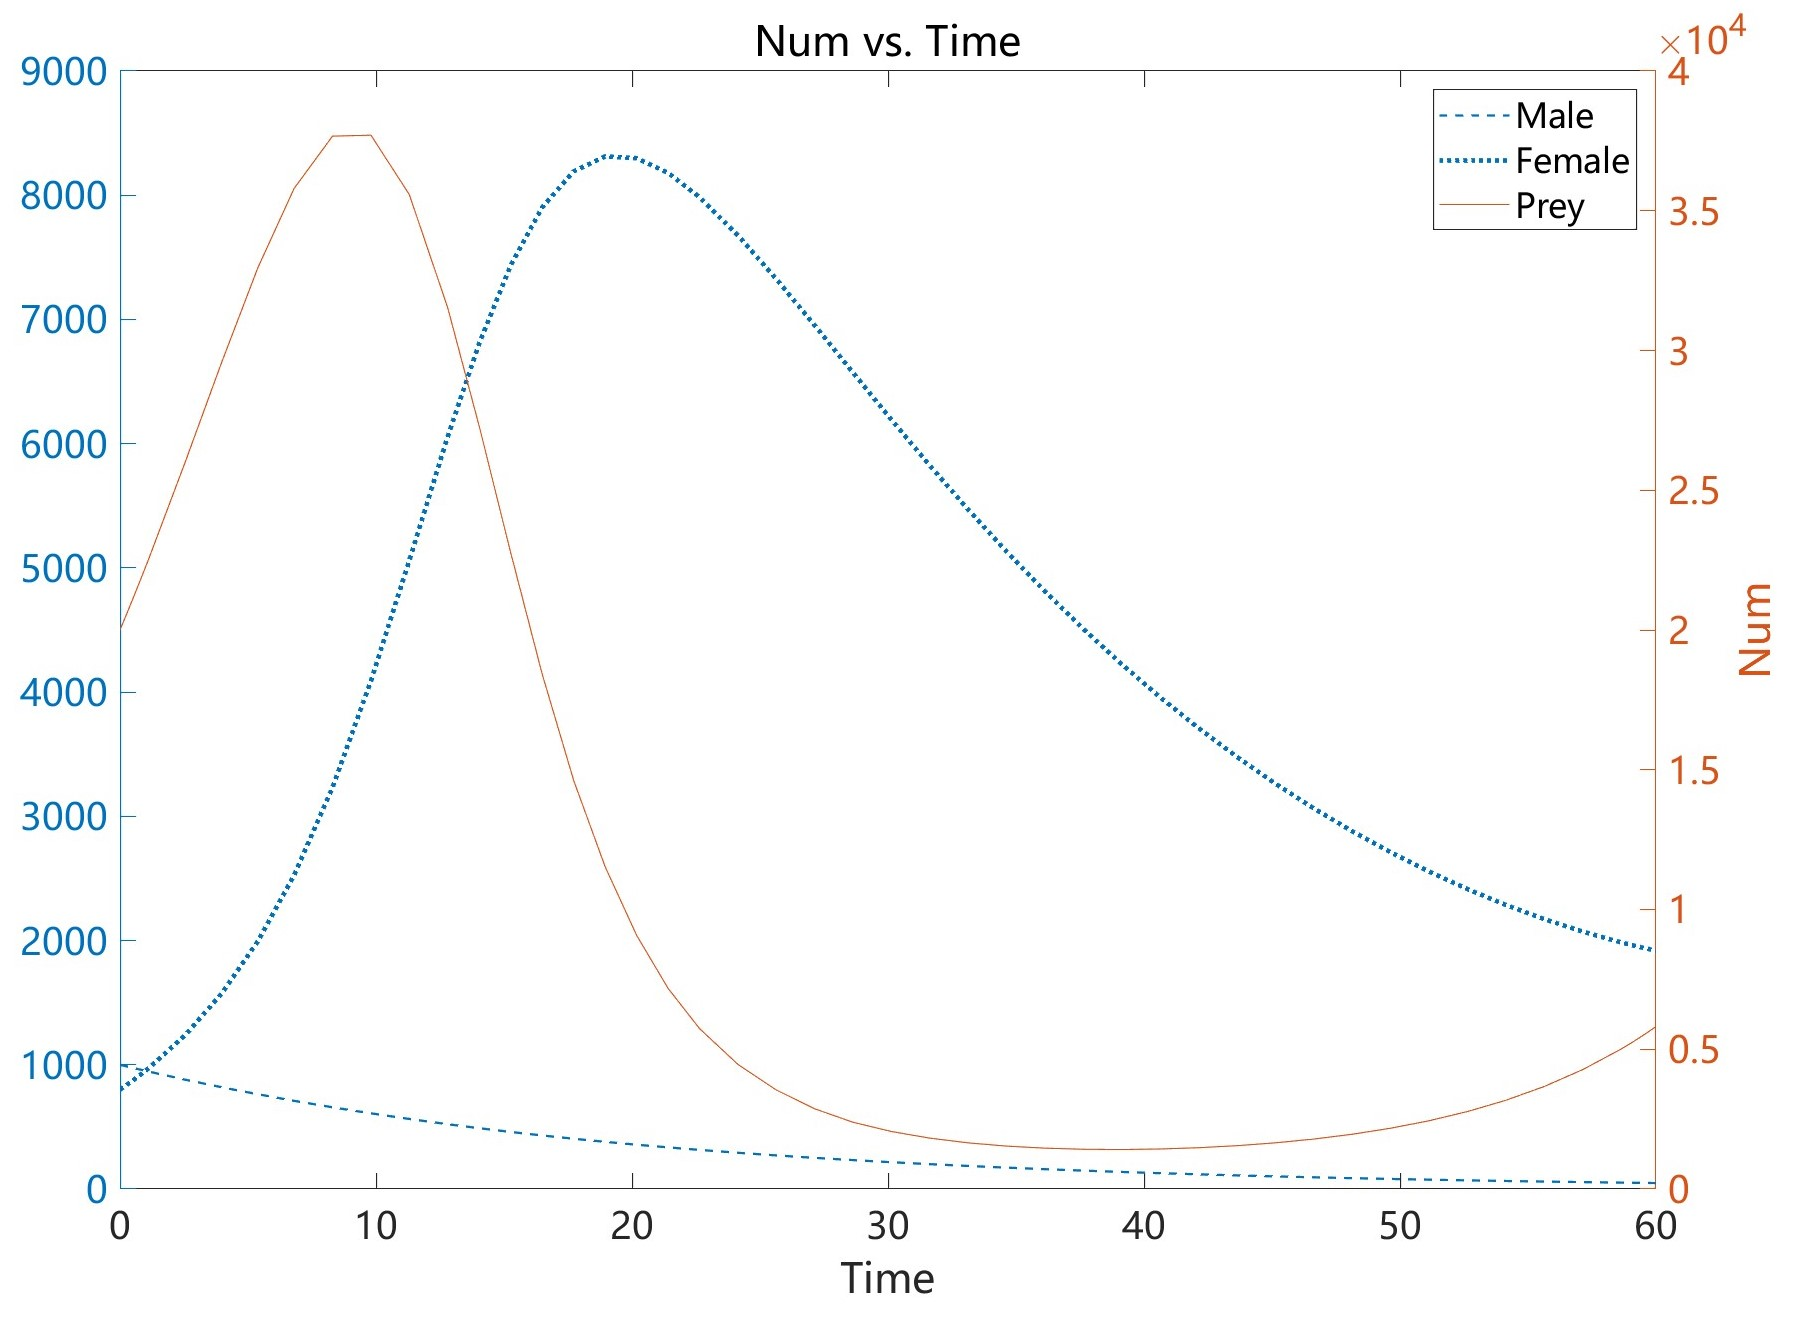
\includegraphics[width=\textwidth]{M2-NumTime-Ext.jpg}\label{M2-NumTime-Ext}
	\end{subfigure}
	\caption{Total extinction of one sex}\label{fig:08}
\end{figure}

\section{Model 3: Sex Ratio Environmental Stability Model with Lyapunov Exponent}
\subsection{Introducing Lyapunov Exponent and Competitors into the System}
Firstly, let's assume a constant gender transition rate, denoted as α. To assess stability, we introduce natural enemies of lampreys (P) and competitors (H). Applying the Lotka-Volterra equation, the partial mortality rate of lampreys in the previous period considered those killed by natural enemies. In this iteration, we refine the mortality rate, comprising natural mortality, competition, and predation rates. The natural mortality is proportional to the lamprey population, the competition rate is proportional to both lamprey and competitor populations, and the predation rate is proportional to the lamprey population and the number of natural enemies.

First, assume that the male differentiation rates is constant as $\alpha$. And to measure this stability, we add the natural enemies of lamprey, the number of which is $P$, and the competitors of lamprey, the number of which is $H$. According to the Lotka–Volterra equation, the mortality rate of lamprey in the previous period has taken into account the number of those who are killed by the natural enemies, therefore, this time, we correct the mortality rate, which is composed of the natural mortality rate, the competition rate, and the rate of predation, the natural mortality rate is proportional to the number of itself, the competition rate is proportional to the number of itself and the number of competitors, the rate of predation is proportional to the number of itself and the number of competitors. The natural mortality rate is proportional to its own number, the competition rate is proportional to its own number and the number of competitors, and the predation rate is proportional to its own number and the number of natural enemies.
\begin{equation}\label{eq:6-1}
\begin{cases}
	\beta N_{M} = \beta_{1}N_{M} + \epsilon_{3}N_{M}P + \theta_{1}a_{M}N_{M}H \\ \\
	\beta N_{F} = \beta_{1}N_{F} + \epsilon_{3}N_{F}P + \theta_{1}a_{F}N_{F}H
\end{cases}
\end{equation}

In the equation, $\theta$ is competition coefficient.
We can get equations for natural enemies and competitors based on the Lotka–Volterra equation:

\begin{equation}\label{eq:6-2}
\begin{cases}
	\frac{\mathrm{d}P}{\mathrm{d}t}=-\beta_{2}P + \epsilon_{4}(a_{1}N_{F}+a_{2}N_{M})P\\ \\
	\frac{\mathrm{d}H}{\mathrm{d}t}=h_{2}H-\theta_{1}(a_{1}N_{F}+a_{2}N_{M})H
\end{cases}
\end{equation}

Combined with the Model 2 (\ref{eq:5-5}) and (\ref{eq:6-2}), we first list the differential equations for this system:


\begin{equation}\label{eq:6-3}
\begin{cases}
	\frac{\mathrm{d}N_{M}}{\mathrm{d}t}=\left( \alpha - \frac{1}{\lambda} \right)\epsilon_{1}U(a)(a_{F}N_{F}+a_{M}N_{M})-\beta_{1}N_{M}-\epsilon_{3}N_{M}P-\theta_{1}a_{M}N_{M}\\
	\\
	\frac{\mathrm{d}N_{F}}{\mathrm{d}t}=\left( 1-\alpha-\frac{1}{\lambda}\right)\epsilon_{1}U(a_{F}N_{F}+a_{M}N_{M})-\beta_{1}N_{F}-\epsilon_{3}N_{F}P-\theta_{1}a_{F}N_{F}\\ \\
	\frac{\mathrm{d}U}{\mathrm{d}t}=hU-\epsilon_{2}U(a_{F}N_{F}+a_{M}N_{M})
\end{cases}
\end{equation}

where $\epsilon$ is the predation conversion coefficient, $\theta$ is the competition conversion coefficient, $h$ is the natural growth coefficient, and $\beta1$ is the natural mortality rate.Combined with the (\ref{eq:6-2}) and (\ref{eq:6-3}),We can get equations:
\begin{equation}\label{eq:6-4}
\begin{cases}
	\frac{\mathrm{d}N_{M}}{\mathrm{d}t}=f(N_{M},N_{F},U,P,H)\\
	\frac{\mathrm{d}N_{F}}{\mathrm{d}t}=g(N_{M},N_{F},U,P,H)\\
	\frac{\mathrm{d}U}{\mathrm{d}t}=h(N_{M},N_{F},U,P,H) \\
	\frac{\mathrm{d}P}{\mathrm{d}t}=\phi(N_{M},N_{F},U,P,H) \\
	\frac{\mathrm{d}U}{\mathrm{d}t}=\rho(N_{M},N_{F},U,P,H)
\end{cases}
\end{equation}

For ease of calculation, we write the unknowns in matrix form:
\begin{equation}\label{eq:6-5}
Y =
\begin{bmatrix}
	M&W&U&P&H
\end{bmatrix}^{T}
\end{equation}

Introducing the Jacobian matrix $J$ which describes the local linear behavior of the system near the equilibrium point:

\begin{equation}\label{eq:6-6}
J = 
\begin{bmatrix}
	\frac{\mathrm{d}f}{\mathrm{d}N_{M}} & \frac{\mathrm{d}f}{\mathrm{d}N_{F}} &\frac{\mathrm{d}f}{\mathrm{d}U} &\frac{\mathrm{d}f}{\mathrm{d}U} &\frac{\mathrm{d}f}{\mathrm{d}U}\\
	\frac{\mathrm{d}g}{\mathrm{d}N_{M}} & \frac{\mathrm{d}g}{\mathrm{d}N_{F}} & \frac{\mathrm{d}g}{\mathrm{d}U} &\frac{\mathrm{d}f}{\mathrm{d}U} &\frac{\mathrm{d}f}{\mathrm{d}U}\\
	\frac{\mathrm{d}h}{\mathrm{d}N_{M}} & \frac{\mathrm{d}h}{\mathrm{d}N_{F}} & \frac{\mathrm{d}h}{\mathrm{d}U} &\frac{\mathrm{d}f}{\mathrm{d}U} &\frac{\mathrm{d}f}{\mathrm{d}U} \\
	\frac{\mathrm{d}f}{\mathrm{d}U}&\frac{\mathrm{d}f}{\mathrm{d}U} &\frac{\mathrm{d}f}{\mathrm{d}U} &\frac{\mathrm{d}f}{\mathrm{d}U} &\frac{\mathrm{d}f}{\mathrm{d}U} \\
	\frac{\mathrm{d}f}{\mathrm{d}U} &\frac{\mathrm{d}f}{\mathrm{d}U} &\frac{\mathrm{d}f}{\mathrm{d}U} &\frac{\mathrm{d}f}{\mathrm{d}U} &\frac{\mathrm{d}f}{\mathrm{d}U}
\end{bmatrix}
\end{equation}

Combined with (\ref{eq:6-4}),(\ref{eq:6-5}) and (\ref{eq:6-6}),we can get the following differential equation:
\begin{equation}\label{eq:6-7}
\frac{\mathrm{d}Y}{\mathrm{d}t}=JY
\end{equation}

The equilibrium point of the system is then calculated assuming $Y_0$ for $\frac{\mathrm{d}Y}{\mathrm{d}t}=0$. The equilibrium point may have $n$ sets of solutions, and we bring the ith set of equilibrium point solutions into the Jacobian matrix to compute the eigenvalue lambda of $J$:

\begin{equation}\label{eq:6-9}
\mid J_{Y_0}-\lambda T\mid = 0
\end{equation}

The equation has a total of $i$ sets of parameters, each of which may have $m$ solutions (usually the values of $m$ and $n$ are equal), and we bring the $j$th solution of the $i$th set of parameters into the formulation of the Lyapunov exponent:

\begin{equation}\label{eq:6-10}
L_{ij}=\lim_{ t \to \infty } 1/t\ln(\mid e^{\lambda_{ij}t}\mid) 
\end{equation}

$L_{ij}$ denotes the Lyapunov exponent under the $j$th eigenvalue of the $i$th group of equilibrium points, and we can know that each group of eigenvalues reflects the stability information of the system near the corresponding equilibrium point according to automatic control theory. We analyze the stability information of the equilibrium point for each group of eigenvalues, and then analyze the stability information of each group of equilibrium points to get the total stability information of the system.
\begin{figure}[htbp]
	\centering
	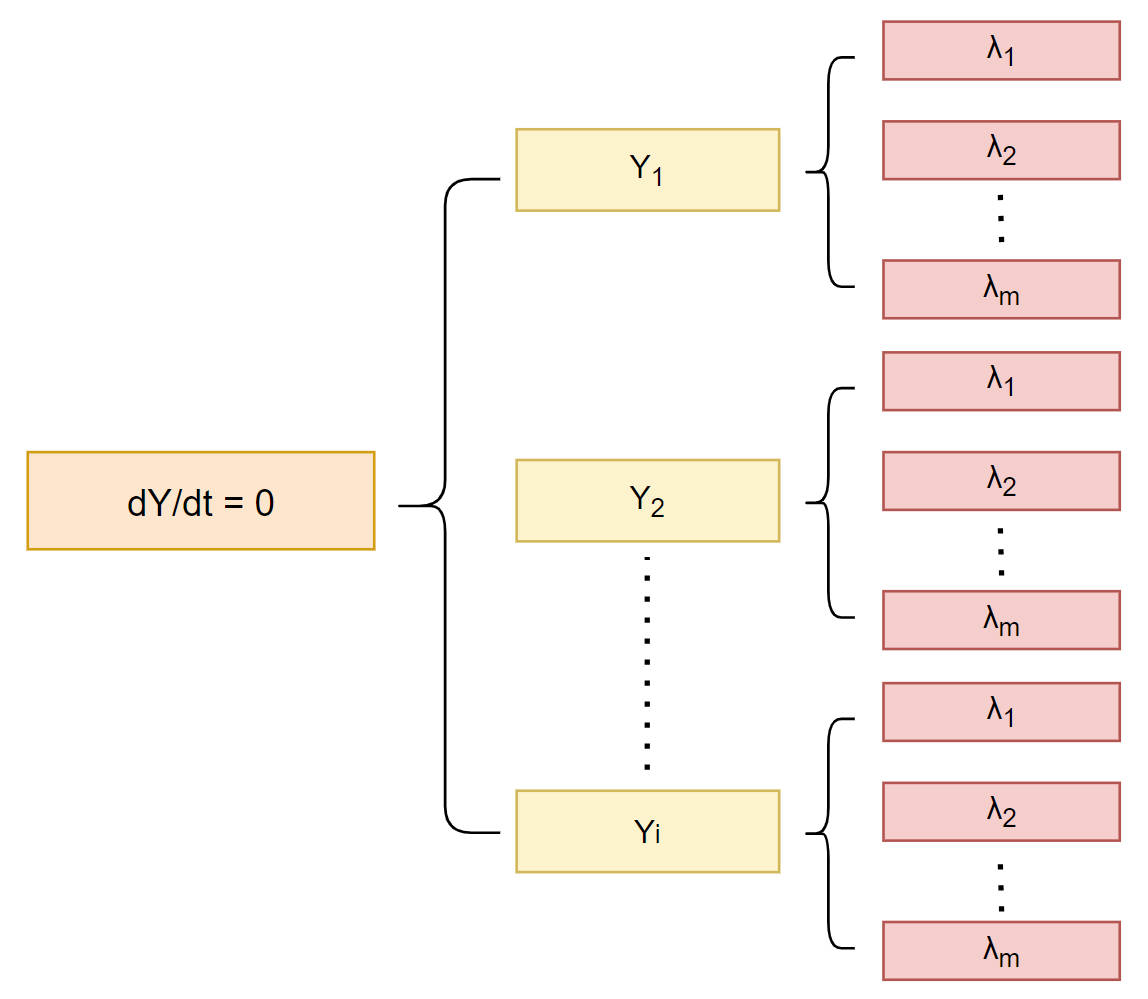
\includegraphics[width=.5\textwidth]{L.jpg}
	\caption{The $\lambda$ of $Y$}\label{fig:L}
\end{figure}

We now obtain the stability of the system at a fixed gender transition coefficient $\alpha$. We then discuss the stability of the system as a varies with the availability of system resources with the help of the Model 1 by adding the time-varying equations:

Redoing the above steps, we can obtain the stability level of the system for fixed $\alpha$ and varying $\alpha$.

\subsection{Analysis of the Result}
According to the literature, when the Lyapunov exponent is negative, the system can maintain stability (cited in the literature), and the larger the absolute value of the value, the faster the reduction of the small disturbance in the system. A smaller absolute value means that the system evolves more slowly. In Figure \ref{LyapunovExponentModel4}, it can be seen that the Lyapunov exponents are all less than zero in any case of α, and so the ecosystem is stable. The small change of a single species will not change the stability of the general environment. As can be seen from Figure \ref{StableNumFixedAlpha}, when the sex ratio of lampreys does not change with the environment, the stability of the system is the best when the sex ratio is 0.44.

In this model, we introduce competition for prey between competitors and lampreys. Lampreys will change the sex ratio of lampreys in response to environmental changes, and the final sex ratio will move up and down around 0.73. (Figure \ref{Model3SexRatio}) This indicates that lampreys choose the strategy of allowing more males to adapt to population growth when food is insufficient. At this time, the Lyapunov exponent reaches -35.1782, which is negative, indicating that the system is stable, and the absolute value is obviously greater than the Lyapunov exponent when the sex ratio is fixed, and the system restores stability faster when it encounters small disturbances. This suggests that sex changes in lampreys enhance the level of balance in the system.

\begin{figure}[htbp]
	\centering
	\begin{subfigure}[b]{.31\textwidth}
		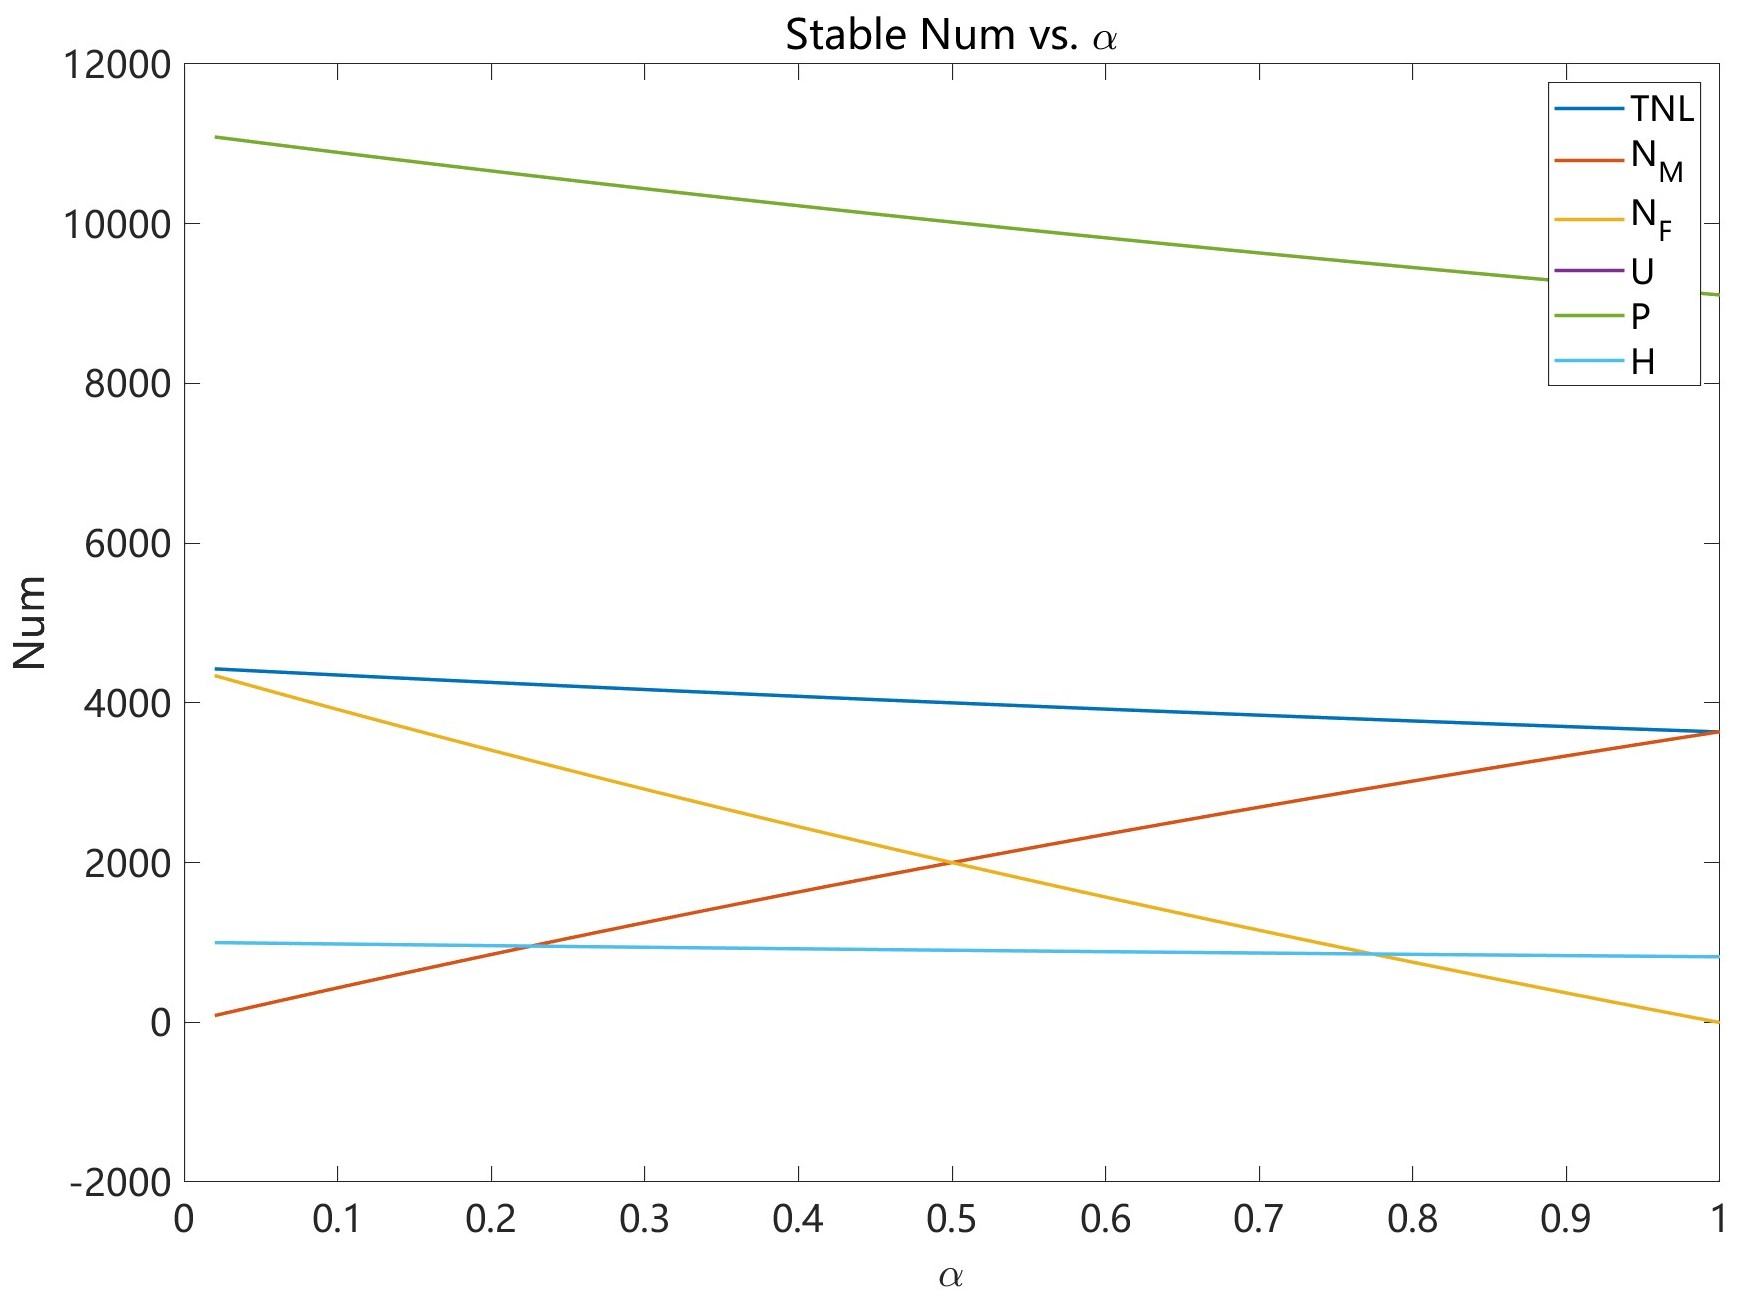
\includegraphics[width=\textwidth]{StableNumFixedAlpha.jpg}
		\caption{\centering Stable population of different $\alpha$ conditions}\label{StableNumFixedAlpha}
	\end{subfigure}
	\begin{subfigure}[b]{.3\textwidth}
		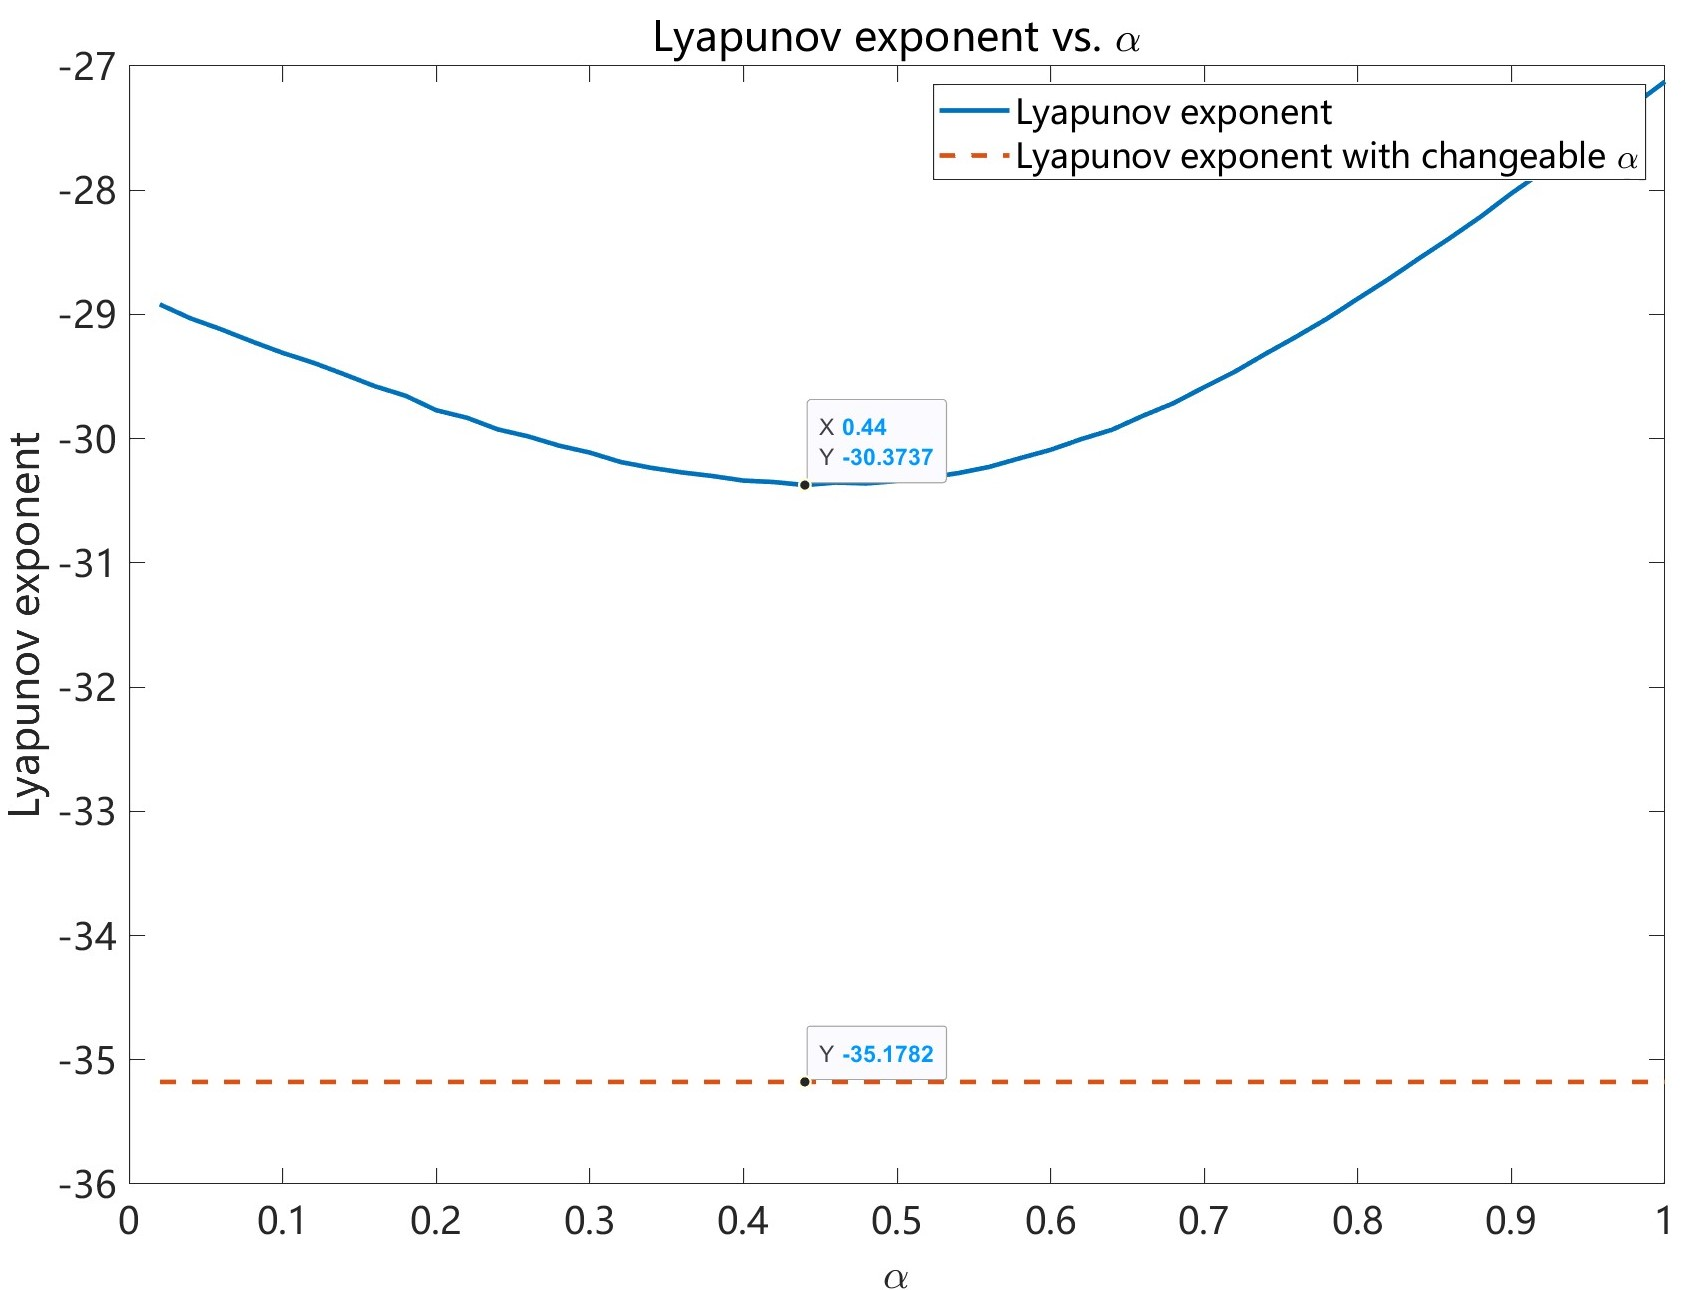
\includegraphics[width=\textwidth]{LyapunovExponentModel4.jpg}
		\caption{\centering Lyapunov Exponents of Different $\alpha$}\label{LyapunovExponentModel4}
	\end{subfigure}
		\begin{subfigure}[b]{.3\textwidth}
		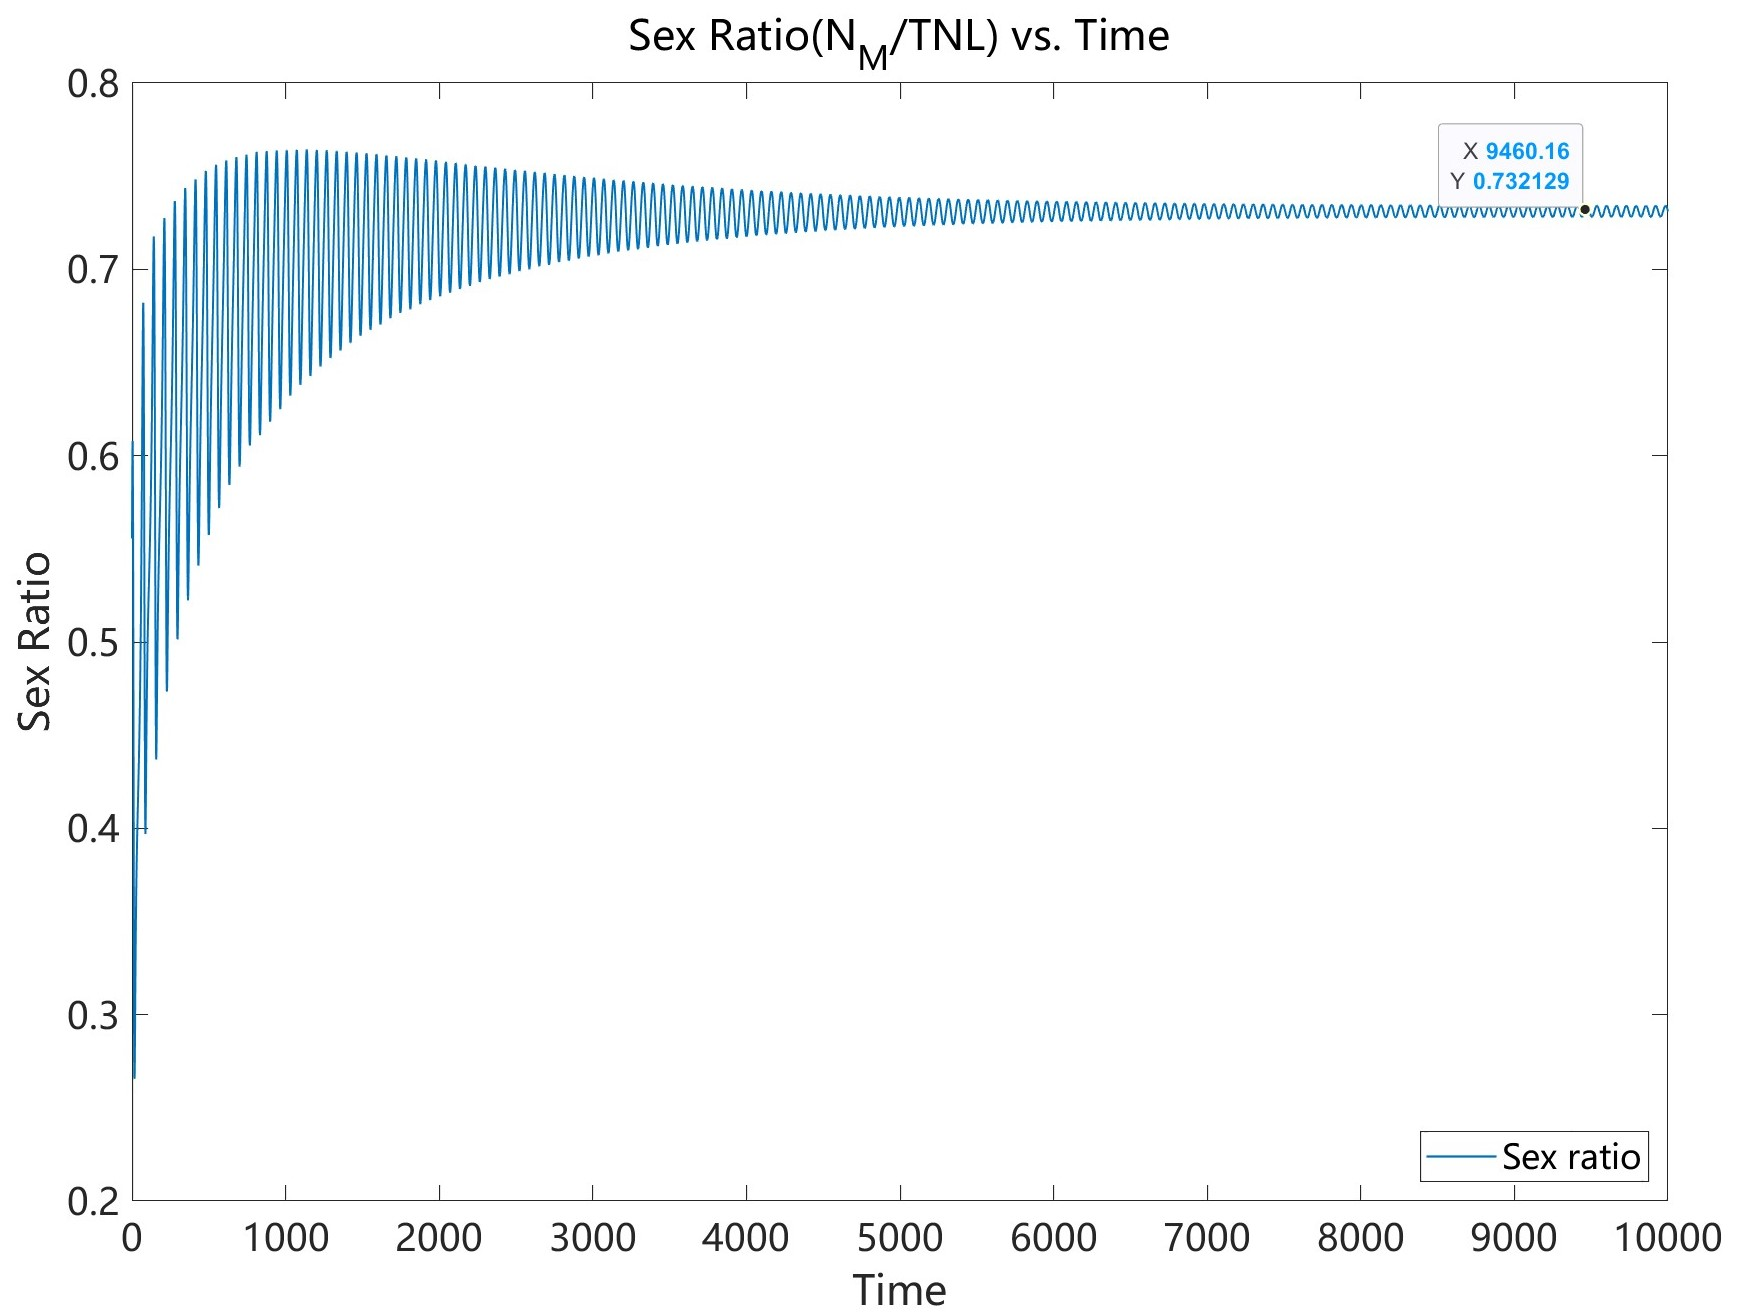
\includegraphics[width=\textwidth]{Model3SexRatio.jpg}
		\caption{\centering Changes in the sex ratio over time}\label{Model3SexRatio}
	\end{subfigure}
	\caption{Lyapunov Exponent of every system}
\end{figure}

\section{Model 4: Population Interaction with Sex Ratios Model}
\subsection{Description of the Transformation From Continuous Food Web Model to Discrete One}
We have included more ecosystem participants as variables in our model in Model 3 (Model 1 and Model 2 assumed them to be constant), so we draw on the differential equation (\ref{eq:6-2}) in Model 3.

It is possible to obtain a schematic representation of the successive changes in species, but this time we consider the effect of the sex ratio of lamprey on the competitors of the lamprey (a.k.a. parasites) as well as the natural enemies of the lamprey and analyze it qualitatively and quantitatively.

When $\alpha$ does not vary as follows, it is shown in Figure \ref{fig:AM3}. When $\alpha$  is varying, the equation is satisfied with (\ref{eq:4-8}) (\ref{eq:4-9}) (\ref{eq:5-1}), We can combine the differential equations above to get the following conclusions:

We can see how sex ratio affects the other participants when the comparison $\alpha$ is not fixed and $\alpha$ is fixed.

Meanwhile, the number of species changes in nature is discrete, and we have once again introduced the metacellular automata for visualization, which facilitates us to understand the process of change more easily. We have already learned about the relationship between lamprey as predator and prey through Model 1 and 2, and now we will only consider the three species, lamprey and competitors as well as natural predators for.

\begin{figure}[htbp]
	\centering
	{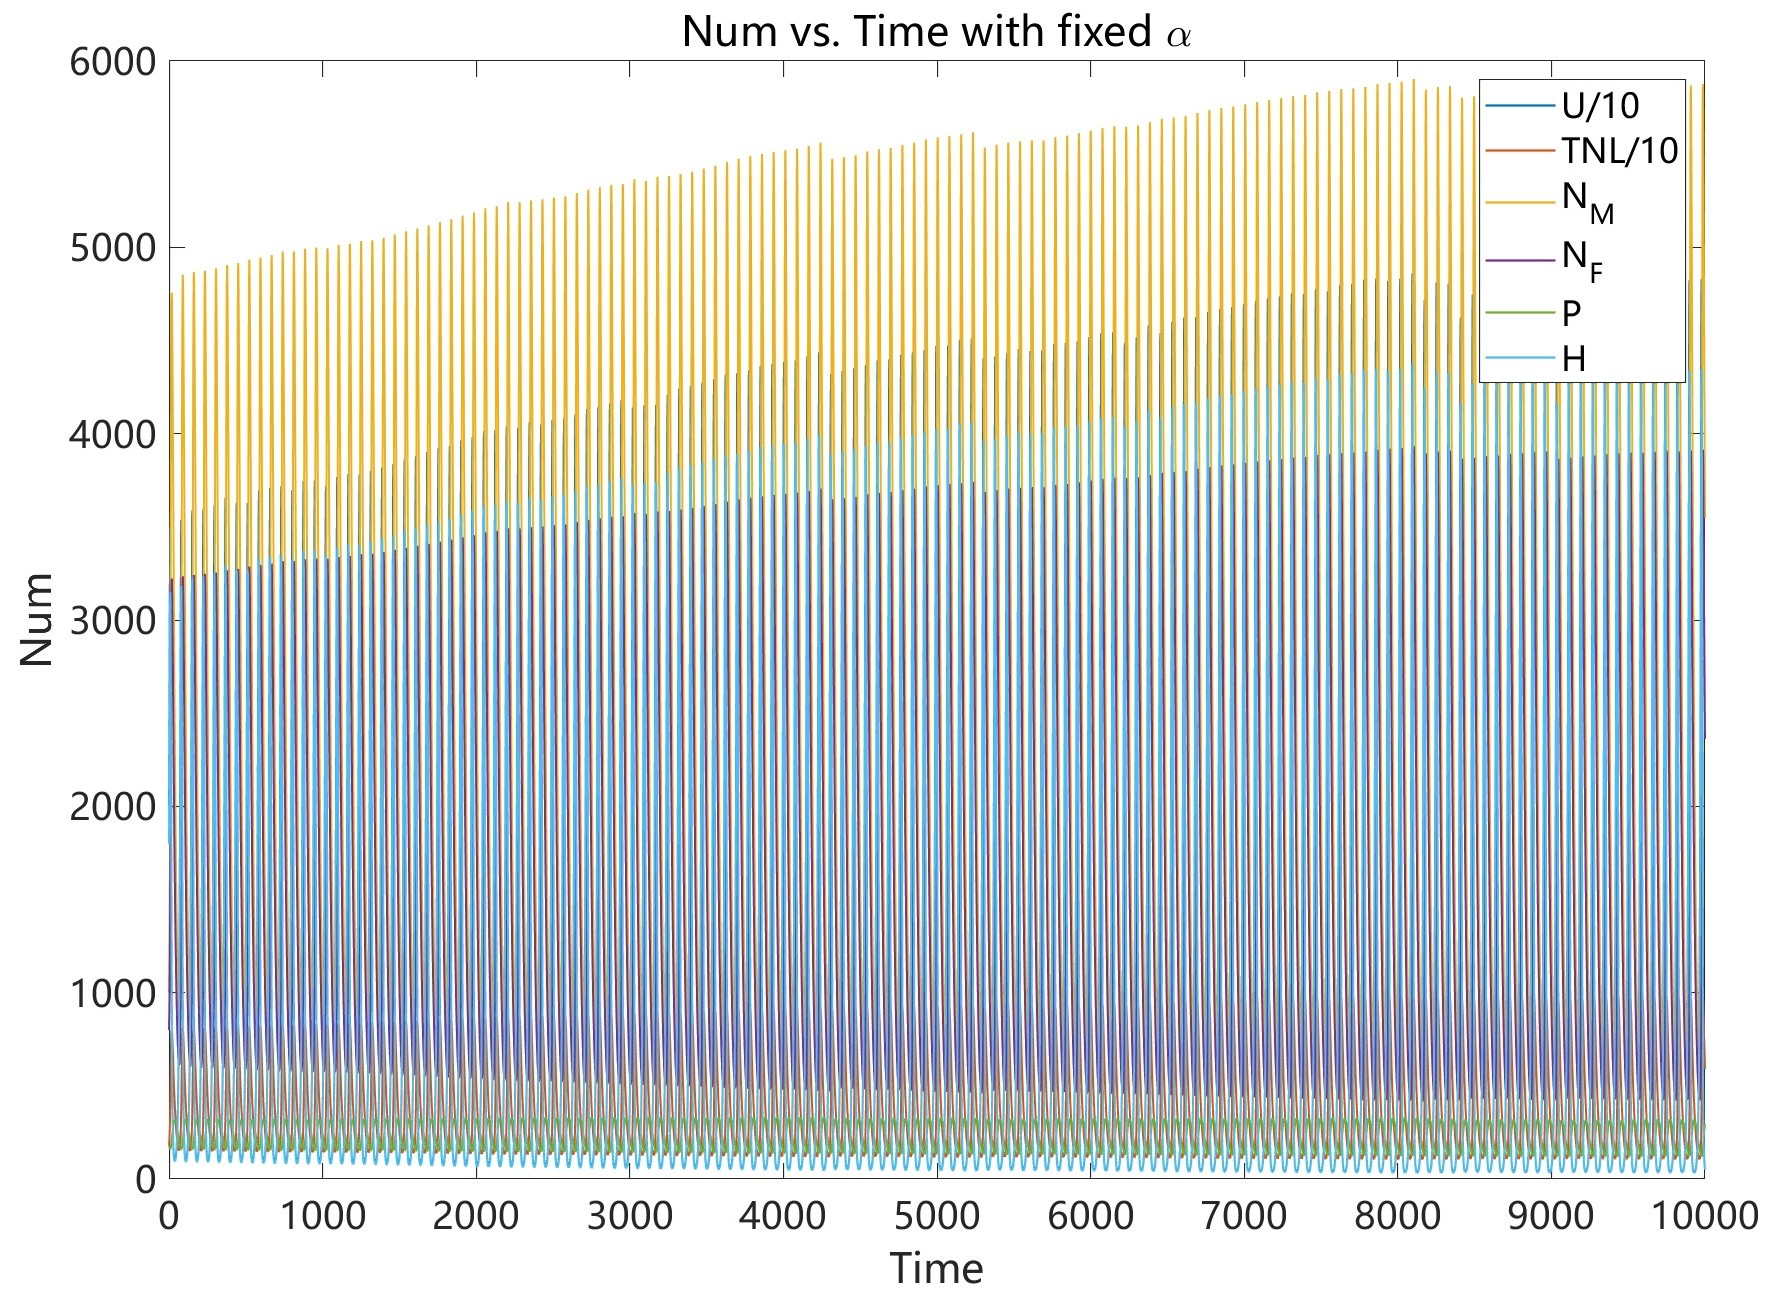
\includegraphics[width=0.45\textwidth]{M4-Num-Time-ExtLong-FixedAlpha.jpg}\label{M4-Num-Time-ExtLong-FixedAlpha}}
	\caption{Changes in population size over time under different $\alpha$}
	\label{fig:AM3}
\end{figure}
In this paper, we discuss the interaction between the three species in two aspects, predation and competition, the parasite and lamprey form a competitive relationship, and the natural enemy and lamprey form a predatory relationship.

Our workload is to quantify these three aspects. We composed the ecosystem in small $n \times n$ cells, and we used a small cell to represent an area, with each cell being a population. When predators and parasites occupy an area, they are affected by the mortality and growth rates of lampreys in the eight surrounding cells, while differences in the sex of the lampreys result in different levels of impact.

For the three populations there are equations for their spread, where $\sigma$ is the spread factor:
\begin{equation}\label{eq:7-1}
\sum\limits_{m=-1}^{1}\sum\limits_{n=-1}^{1}P_{i+m,j+m}(t+\Delta t) = \sigma P_{ij}(t)
\end{equation}
Spreading factor is the proximity rule coefficient of the metacellular automaton, related to predation and competition, it also shows the species under the ecosystem, and is equal to the growth rate minus the mortality rate.

The growth rate is the natural rate of growth plus the rate associated with other populations, and the mortality rate is the natural rate of death plus the rate associated with other populations. Based on the partial analysis of the previous Model 3, we derive the four dispersal factors and make the overall dynamic equation:
\begin{equation}\label{eq:7-2}
\begin{cases}
	\sum\limits_{m=-1}^{1}\sum\limits_{n=-1}^{1}P_{i+m,j+m}(t+\Delta t) = [(\sigma_{1}-\beta_{1}) + K_{1}(a_{F}F_{ij}(t) + a_{M}M_{ij}(t))]P_{ij}(t)\\
	\sum\limits_{m=-1}^{1}\sum\limits_{n=-1}^{1}H_{i+m,j+m}(t+\Delta t) = [(\sigma_{2}-\beta_{2}) - K_{2}(a_{F}F_{ij}(t) + a_{M}M_{ij}(t))]H_{ij}(t) \\
	\sum\limits_{m=-1}^{1}\sum\limits_{n=-1}^{1}N_{Fi+m,j+m}(t+\Delta t) = [(b_{3}\alpha-\beta_{3}) - K_{4}a_{F}P_{ij}(t) - K_{5}a_{M}H_{ij}(t)]N_{Fij}(t) \\
	\sum\limits_{m=-1}^{1}\sum\limits_{n=-1}^{1}N_{Mi+m,j+m}(t+\Delta t) = [(b_{3}(1-\alpha)-\beta_{3}) - K_{4}a_{M}P_{ij}(t) - K_{5}a_{F}H_{ij}(t)]P_{ij}(t)
\end{cases}
\end{equation}
In summary, we obtain by matlab simulation:
\begin{figure}[htbp]
	\centering
	\subfloat[]
	{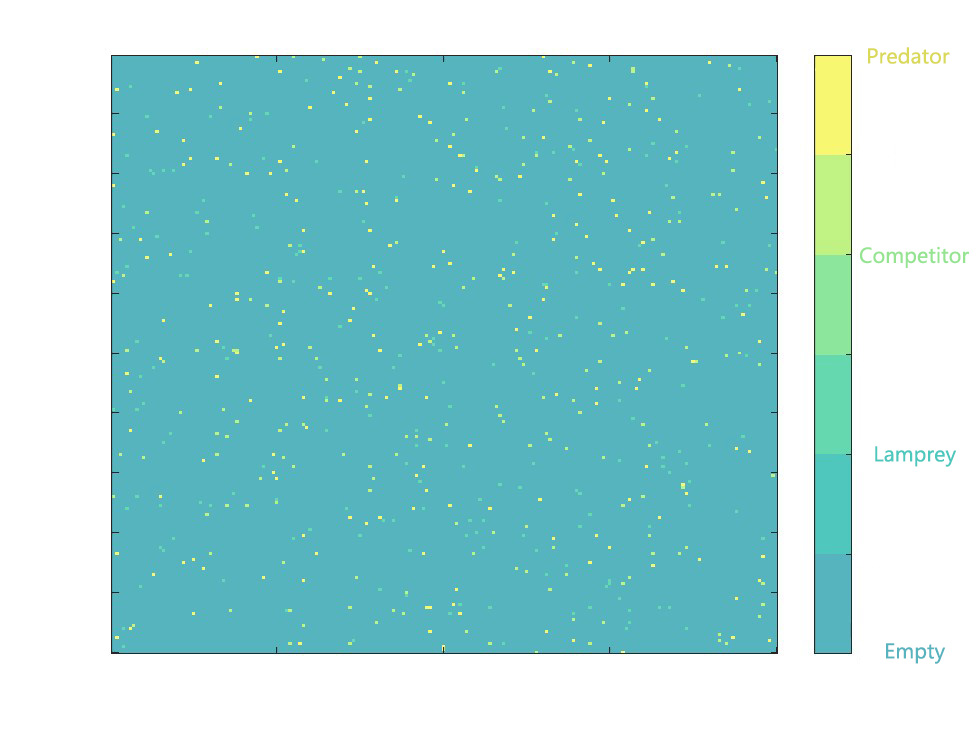
\includegraphics[width=0.35\textwidth]{Cell1-Done.jpg}\label{Cell1-Done}}
	\quad
	\subfloat[]
	{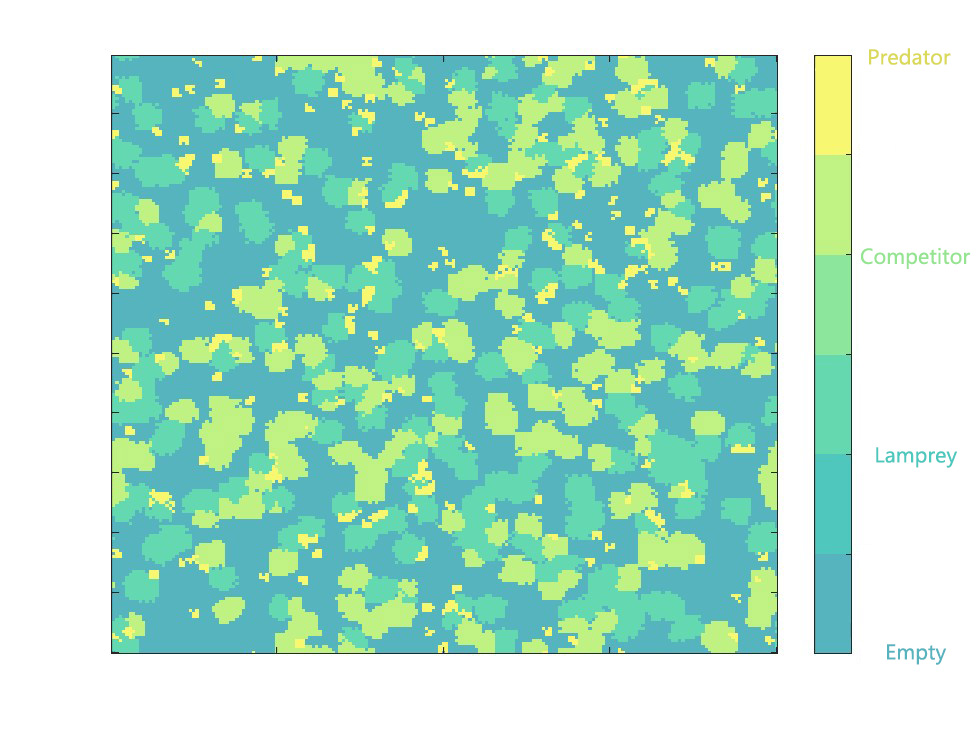
\includegraphics[width=0.35\textwidth]{Cell2-Done.jpg}\label{Cell2-Done}}
	\quad
	\subfloat[]
	{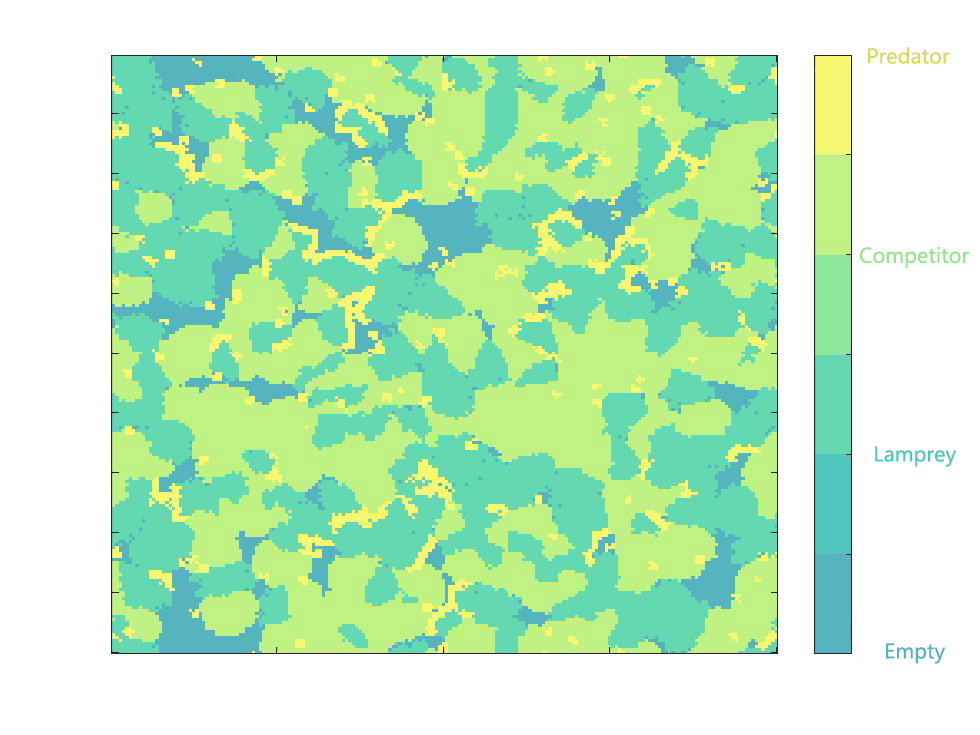
\includegraphics[width=0.35\textwidth]{Cell3-Done.jpg}\label{Cell3-Done}}
	\quad
	\subfloat[]
	{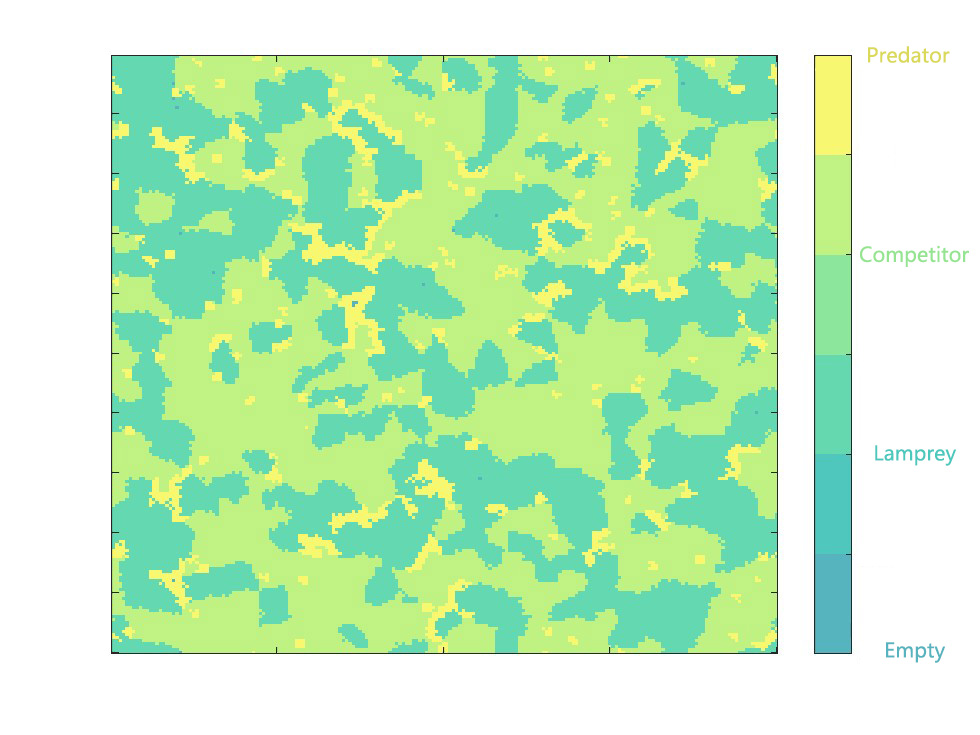
\includegraphics[width=0.35\textwidth]{Cell4-Done.jpg}\label{Cell4-Done}}
	\quad
	\caption{Metacellular automata evolution diagram} \label{fig:AM}
\end{figure}

\subsection{Analysis of the Result}

By analyzing Figure \ref{M4-Num-Time}, it is evident that the population curves of prey and competitors exhibit a cooperative relationship. As the number of prey increases, so does the number of competitors. Conversely, as prey numbers decline, competitor populations also decrease; however, the rate of decline surpasses the previous rate of increase. 

Furthermore, Figure \ref{M4-Num-Time-SexRatio} illustrates that lamprey sex ratios consistently range between 0.56 and 0.78. When prey numbers decrease, the sex ratio increases while lamprey populations decline gradually. On the other hand, when prey numbers increase, the sex ratio decreases and lamprey populations experience rapid growth. This adaptability and competitiveness enable lampreys to thrive in their ecosystem. Additionally observed in Figure \ref{M4-Num-Time} is a lag in total lamprey population compared to competitor population curves. Competitors maintain a fast growth rate when their numbers are high but gradually decrease as lampreys begin to multiply. This indicates that lampreys possess significant competitive abilities within this model's ecosystem. 

Consequently, it becomes easier for lampreys to dominate most available food resources within this ecosystem context leading to reduced competitor populations due to limited food availability—explaining why competitors decline at a faster rate than they grow and placing them at risk of extinction. These circumstances shed light on why lampreys have survived throughout history and emphasize why intervention from organizations like the Great Lakes Fishery Commission \cite{6} is necessary for controlling their numbers in order to protect other species within this ecosystem. Regarding predators, an abundance of lampreys promotes predator population growth—a trend also depicted in Figure \ref{M4-Num-Time} where predator populations grow fastest when there is a peak in Lamprey abundance and decline rapidly during periods with minimal Lamprey presence.
\begin{figure}[htbp]
	\centering
	\subfloat[]
	{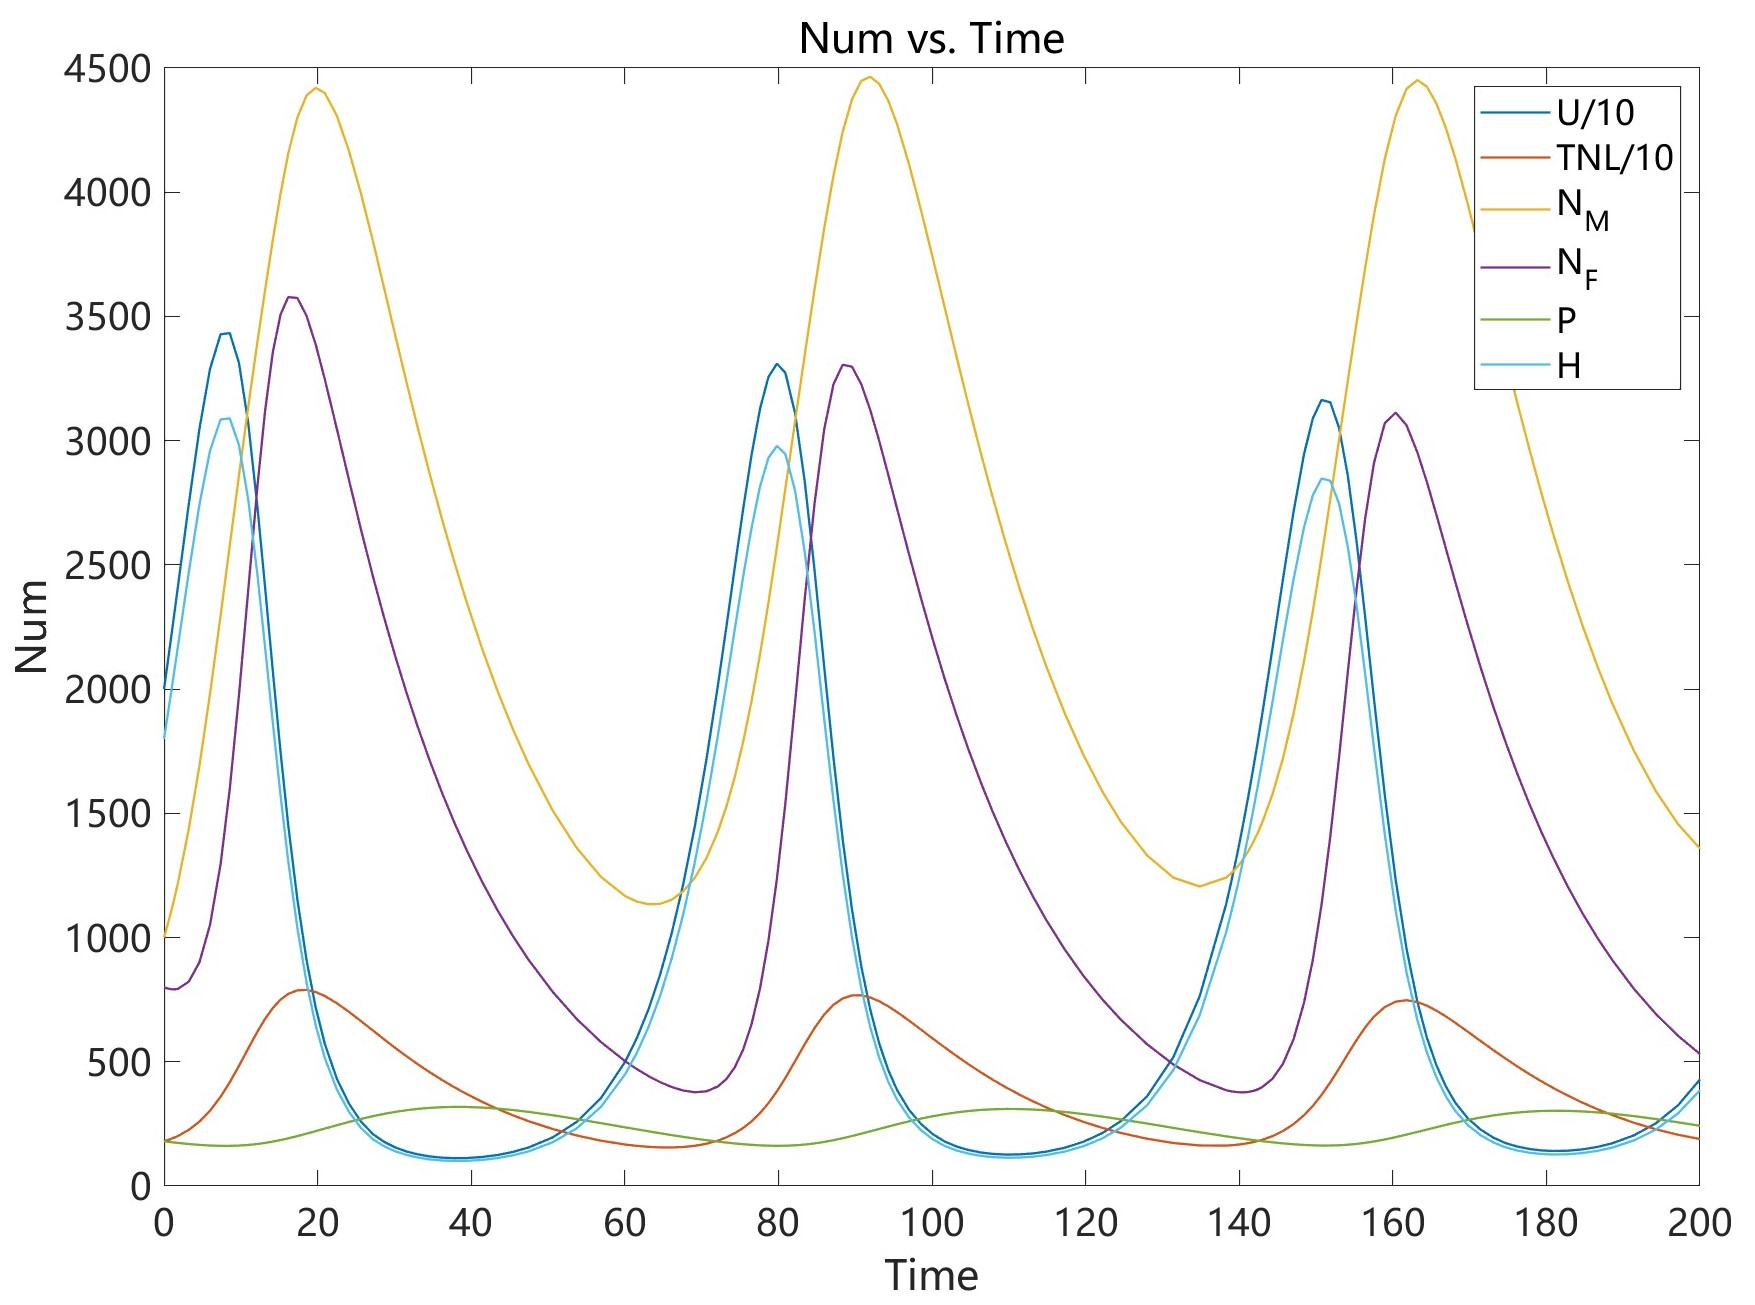
\includegraphics[width=0.3\textwidth]{M4-Num-Time.jpg}\label{M4-Num-Time}}
	\quad    % 重点就在这,优先横向排列,自动换行
	\subfloat[]
	{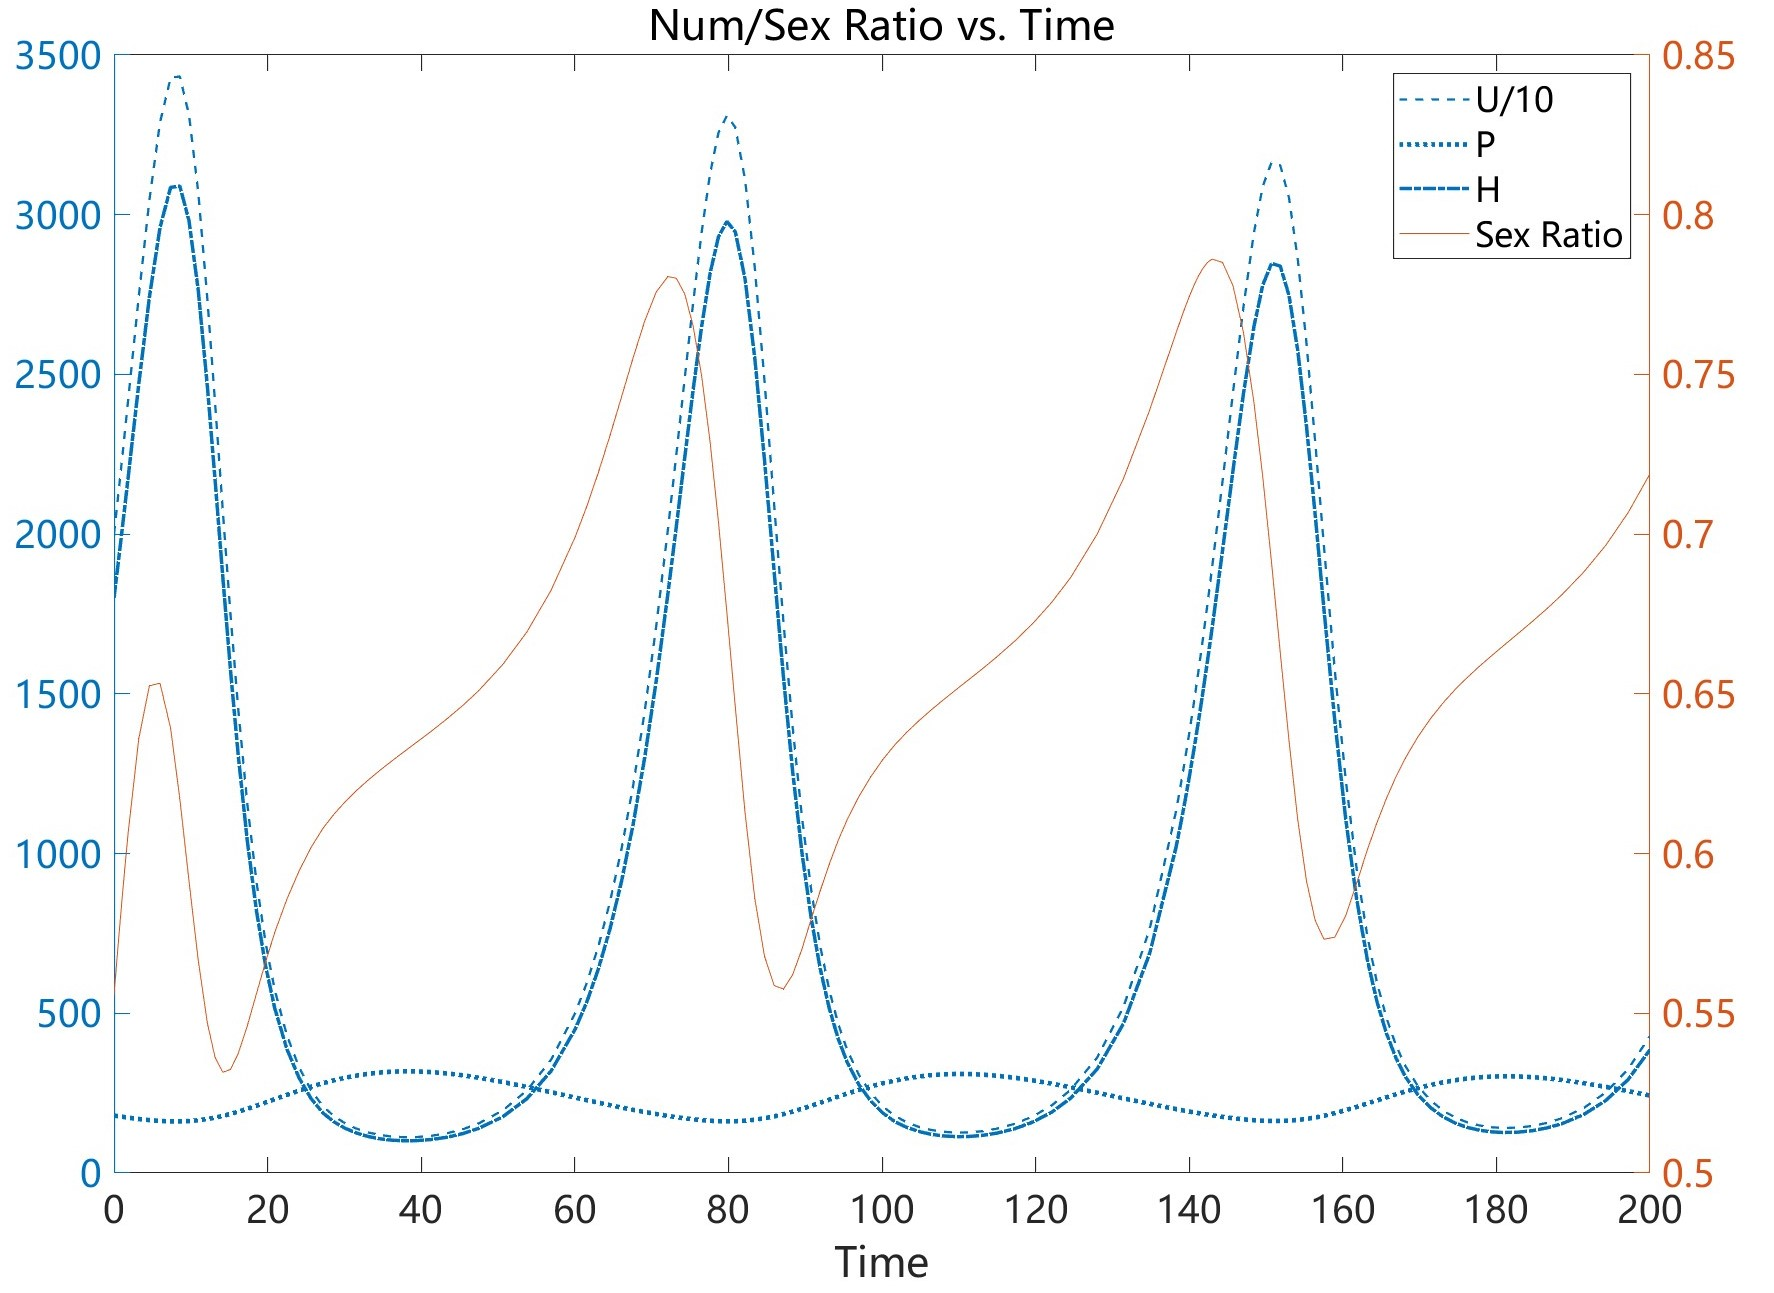
\includegraphics[width=0.3\textwidth]{M4-Num-Time-SexRatio.jpg}\label{M4-Num-Time-SexRatio}}
	\quad
	\subfloat[]
	{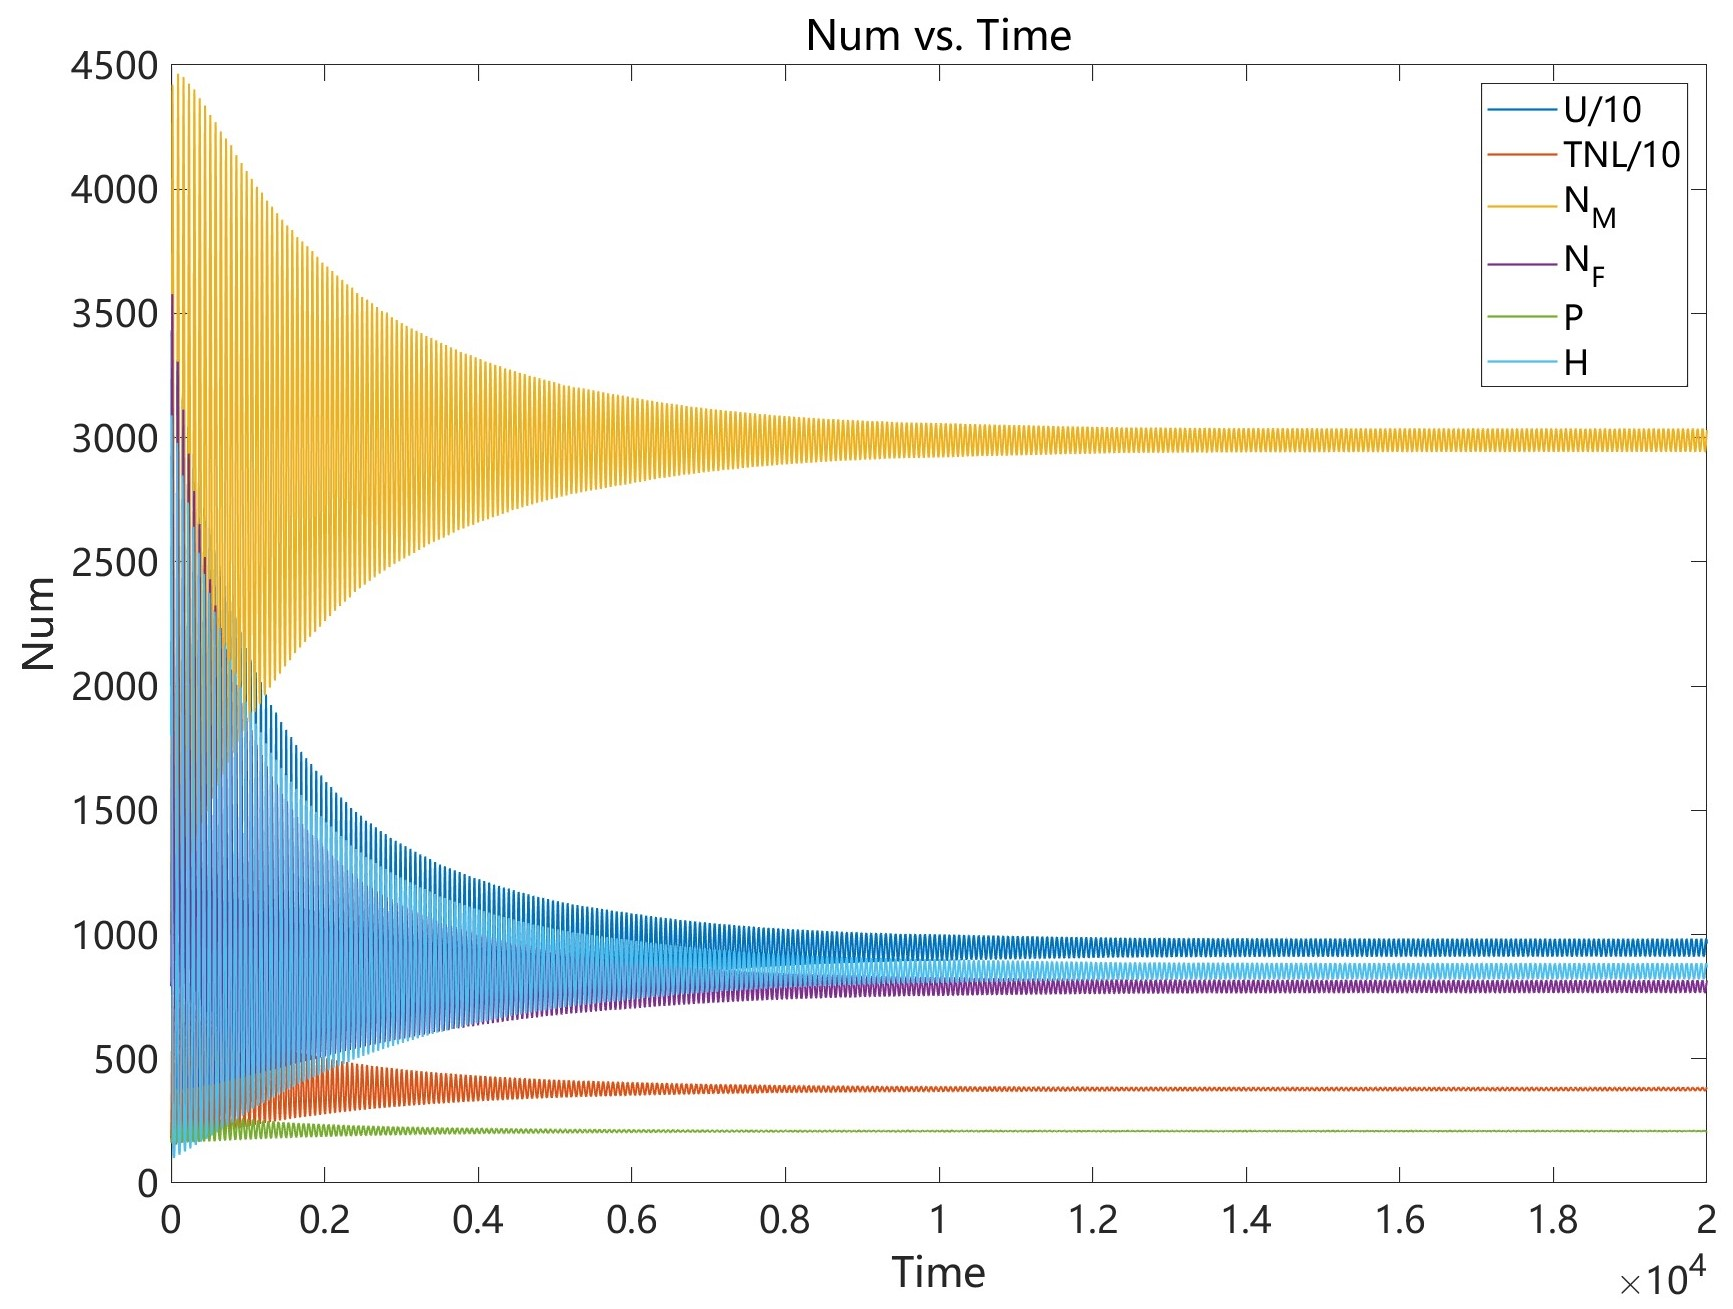
\includegraphics[width=0.3\textwidth]{M4-Num-Time-Long.jpg}\label{M4-Num-Time-Long}}
	\quad
	\caption{The variation of various curves over time} \label{fig:AM4}
\end{figure}


\section{Test the Model}

\subsection{Stability Analysis}
In our simulation of the metacellular automaton, the initial populations are generated randomly and several simulation experiments are carried out, and it is found that the final images obtained are similar and the conclusions are the same, indicating that our final model has good stability.

\subsection{Sensitivity Analysis}
In an ecosystem, the mortality rate of a species is an important indicator that affects the ecological environment. Obviously, the higher the mortality rate of lampreys, that is, the higher the negative feedback of the environment, the more stable the corresponding system will be, and the smaller the corresponding Lyapunov exponent, as mentioned above. When calculating the Lyapunov exponent for this model while varying the mortality rate, it is observed that a negative correlation trend emerged, aligning with real-world observations and successfully passing sensitivity tests. This outcome further validates both the rationality and robustness of this model.
\begin{table}[!htbp]
	\begin{center}
		\begin{threeparttable}
			\caption{The data of sea lamprey}
			\begin{tabular}{cc}
				\toprule
				\multicolumn{1}{m{6cm}}{\centering Rate of change of $\beta$}
				&\multicolumn{1}{m{6cm}}{\centering The Lyapunov exponent} \\
				\midrule
0 & -29.259  \\ 
0.015 & -32.432 \\ 
0.030 & -35.265  \\ 
0.045 & -34.690  \\ 
0.070 & -37.213  \\ 
				
				\bottomrule
			\end{tabular}
			\small
		\end{threeparttable}
	\end{center}
\end{table}

\begin{figure}[htbp]
	\centering
	{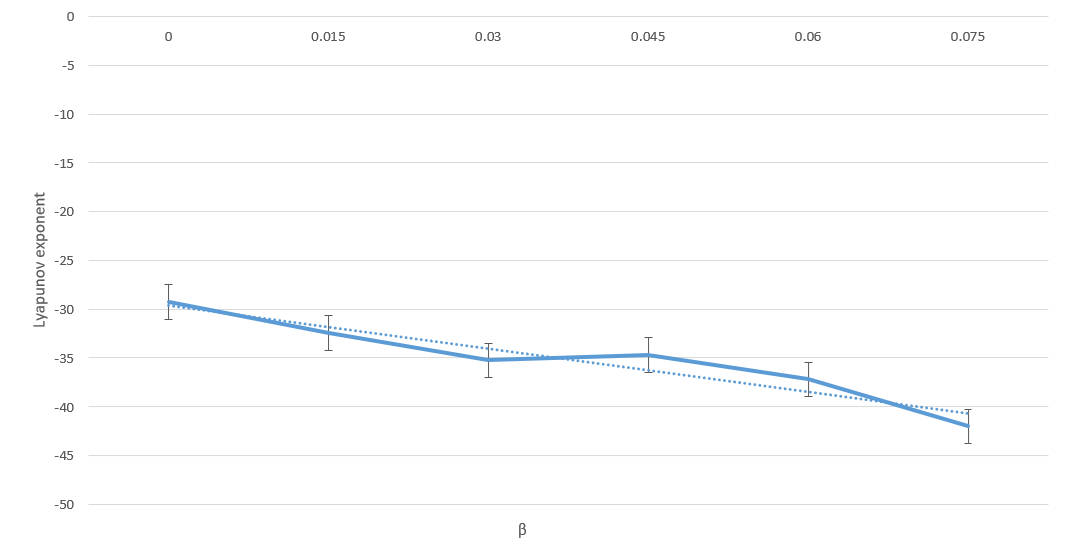
\includegraphics[width=0.6\textwidth]{Sensitivity analysis of β and L.jpg}\label{Sensitivity analysis of β and L}}
	\caption{Sensitivity analysis of β and  Lyapunov exponent}
	\label{fig:AM5}
\end{figure}

\section{Model Conclusion }

\subsection{Summary of Results}
\subsubsection{Summary for Model 1}
Introducing the concept of environmentally available resources, the study found that variable sex ratios allow lamprey populations to utilize resources more and allow for lower resource availability in larger ecosystems.
\subsubsection{Summary for Model 2}
Introducing the concept of predators and examining this food chain, it is found that variable sex ratios have the advantage of increasing the number of males who are better able to adapt to the environment when resources are scarce, allowing the population to cope with greater environmental pressures, and increasing the number of females who are better able to reproduce and take up resources when resources are plentiful, allowing the population to take up a greater share of the resources in the ecosystem.
\subsubsection{Summary for Model 3}
The introduction of predators and competitors that form a typical food web allows the model to describe an ecosystem that can be studied, thus introducing the Lyapunov exponent of automated control theory, which is found to change the sex ratio of lampreys, allowing for greater ecosystem stability.
\subsubsection{Summary for Model 4}
On the basis of model 3, the model is discretized to make it more consistent with the real law of reproduction within populations, and metacellular automata are introduced to describe the interactions among populations in the whole ecosystem, and it is finally found that in ecosystems with variable sex ratios in the lamprey population, the greater stability of the lamprey population led to greater stability of the other populations as well, and is visualized with metacellular automata.

\subsection{Strengths and Possible Improvements}

\subsubsection{Strengths}
\begin{itemize}
	\item Discarding the factors that have less influence and retaining the factors that have more influence on the population of lampreys, the relationship between the sex ratio and the number of lampreys is established on the basis of differential equations, and the results are in good agreement with the actual results.
	\item Creatively, the Lyapunov exponent in the field of automatic control is introduced to measure the stability of the overall ecosystem, and the discrete analysis is carried out by cellular automata to make it more in line with the reality, and various influences of lampreys on the ecosystem are successfully explained.
\end{itemize}

\subsubsection{Possible Improvements}


\begin{itemize}
	\item This model is based on the convenience of arithmetic, model complexity considerations, only consider three typical populations constitute two typical relationships, but in fact, the natural world has more populations, but also in the existence of mutualistic symbiosis and other more complex relationships.
	\item The model ignores the transformation of external energy by producers, and considers that the material and energy of the system always remain stable, that is, the total amount of available resources remains unchanged, but in fact, the ecosystem is not an isolated system, and there are influences of external material and energy.
\end{itemize}



\newpage
% 参考文献,此处以 MLA 引用格式为例
\begin{thebibliography}{99}
\bibitem{1} Karlin S, Lessard S. Theoretical studies on \emph{sex ratio evolution}[J]. 1986.
\bibitem{2} Almeida P R, Arakawa H, Aronsuu K, et al. \emph{Lamprey fisheries: History, trends and management}[J]. Journal of Great Lakes Research, 2021, 47: S159-S185.
\bibitem{3} \emph{The National Center for Biotechnology Information: sea lamprey}, from\url{https://www.ncbi.nlm.nih.gov/pmc/articles/PMC5378093/}
\bibitem{4} Lewandoski, S. A. Brenden, T. O. (2022). Forecasting suppression of invasive sea lamprey in Lake Superior. Journal of Applied Ecology, 59, 2023–2035. from \url{https://doi.org/10.1111/1365-2664.14203}
\bibitem{5} Assembly, ecosystem functions, and stability in species interaction networks LI Hai-Dong, WU Xin-Wei, XIAO Zhi-Shu from \url{https://www.plant-ecology.com/article/2021/1005-264X/1005-264X-45-10-1049.shtml}
\bibitem{6} The data in Great Lakes Fishery Commission from \url{https://www.glfc.org/pubs/slcp/annual_reports/ANNUAL_REPORT_2022.pdf}
\bibitem{7} William D. Swink,Host Selection and Lethality of Attacks by Sea Lampreys (Petromyzon marinus) in Laboratory Studies,Journal of Great Lakes Research,Volume 29, Supplement 1,2003,Pages 307-319,ISSN 0380-1330, from \url{https://doi.org/10.1016/S0380-1330(03)70496-1}
\bibitem{8} G.J Farmer, F.W.H Beamish, G.A Robinson,
Food consumption of the adult landlocked sea lamprey, Petromyzon marinus, L.,
Comparative Biochemistry and Physiology Part A: Physiology,Volume 50, Issue 4,1975,Pages 753-757,ISSN 0300-9629, from \url{https://doi.org/10.1016/0300-9629(75)90141-3.}
\bibitem{9} Khan, Arfa Investigation of candidate sex determination and sex differentiation genes in sea lamprey, Petromyzon marinus, and Pacific lamprey, Entosphenus tridentatus from \url{https://mspace.lib.umanitoba.ca/items/6ebb6260-7784-45a0-bd52-8ec9083ec42d}
\bibitem{10} Docker, M.F., Beamish, F.W.H. (1994). Age, growth, and sex ratio among populations of least brook lamprey, Lampetra aepyptera, larvae: an argument for environmental sex determination. In: Balon, E.K., Bruton, M.N., Noakes, D.L.G. (eds) Women in ichthyology: an anthology in honour of ET, Ro and Genie. Developments in environmental biology of fishes 15, vol 15. Springer,Dordrecht. from \url{https://doi.org/10.1007/978-94-011-0199-8_16}
\bibitem{11} When sex differences lead to extinction from \url{https://www.nature.com/articles/d41586-018-04059-7}
\end{thebibliography}

% 以下为附录内容
% 如您的论文中不需要附录,请自行删除
\begin{subappendices}  % 附录环境

\section{Appendix: Source Code on the Model}
Here are the program codes we used in our research.
% MATLAB 代码示例
\begin{lstlisting}[language=MATLAB, name={test.m}]
% Lyapunov Exponents
syms M W U P H;
y0 = fsolve(@(t) lampreyModel4(t,Ram),[1000,800,20000,180,1800]);
f = @(M,W,U,P,H) ((0.56+(Ram-(epsilon1*U*(a1*W+a2*M)/(c*W*M/...
(W+M)^2)))/(Ram)*0.4)-1/lambda)*epsilon1*U*(a1*W+a2*M)-beta1*M;
g = @(M,W,U,P,H) (1-(0.56+(Ram-(epsilon1*U*(a1*W+a2*M)/...
(c*W*M/(W+M)^2)))/(Ram)*0.4)-1/lambda)*epsilon1*U*(a1*W+a2*M)-beta1*W;
k = @(M,W,U,P,H) -epsilon2*U*(a1*W+a2*M)+h1*U;
m = @(M,W,U,P,H) -beta2*P + epsilon4*(a1*W+a2*M)*P;
n = @(M,W,U,P,H) h2*H-theta2*(a1*W+a2*M)*H;
F = [f(M,W,U,P,H); g(M,W,U,P,H); k(M,W,U,P,H);...
m(M,W,U,P,H); n(M,W,U,P,H)];
J = jacobian(F, [M, W, U, P, H]);
J_eq = double(subs(J, [M, W, U, P, H], y0));
eigenvalues = eig(J_eq);
lyapunov_exponents = real(log(abs(eigenvalues)));

% Part of Cell Auto Machine
% State transition function
function new_blocks = applyRule(blocks)
% move
for i = 1:200
for j = 1:200
num = blocks(i,j,2);
if(num<1)
continue;
end
moveNum = movePos(num);
whe = randi([0,1]);
if(whe&&blocks(stdIndex(i+1),stdIndex(j+1),1)==0||...
blocks(stdIndex(i+1),stdIndex(j+1),1)==blocks(i,j,1))
blocks(stdIndex(i+1),stdIndex(j+1),8) =...
blocks(stdIndex(i+1),stdIndex(j+1),8) + moveNum(7);
blocks(i,j,8) = blocks(i,j,8) - moveNum(7);
blocks(stdIndex(i+1),stdIndex(j+1),1) = blocks(i,j,1);
end
% ... And other 7 direction
end
end
for i = 1:200
for j = 1:200
blocks(i,j,2) = blocks(i,j,2) + blocks(i,j,8);
blocks(i,j,8) = 0;
end
end
% parameter 
% ...
% Calculate all parameter
for i = 1:200
for j = 1:200
if(blocks(i,j,1)==0)
continue;
end
if(blocks(i,j,1)==1)
blocks(i,j,5) = genderC*findBlockNum(i,j,blocks,0); % sex ratio
blocks(i,j,3) = blocks(i,j,5)*lampreyIncC1 + lampreyIncC2; 
% increasing ratio
blocks(i,j,6) = bePredation*findBlockNum(i,j,blocks,3); % be prey ratio
blocks(i,j,7) = beComplete*findBlockNum(i,j,blocks,2); 
% be complete ratio
blocks(i,j,4) = deathBeCom*blocks(i,j,7) +
deathBePre*blocks(i,j,6) + deathLamprey; % death ratio
blocks(i,j,2) = blocks(i,j,2) +
blocks(i,j,2)*(blocks(i,j,3)-blocks(i,j,4));
end
% ... And blocks(i,j,2),blocks(i,j,3)
end
end
new_blocks = blocks;
end


% Model 3&4
function dydt = lampreyModel4(t,y,Ram)
dydt = zeros(5,1);
% y(1)是M,y(2)是F,y(3)是U,y(4)是P,y(5)是H
%parameter
epsilon1 = 0.000005;epsilon2 = 0.00005;epsilon3 = 0;epsilon4 = 0.00001;
a1 = 0.9;a2 = 1.1;beta1 = 0.05;beta2 = 0.04;lambda = 1000;c = 1;
theta1 = 0;theta2 = 0.00005;h1 = 0.2;h2 = 0.2;
r = c*y(2)*y(1)/(y(1)+y(2))^2;
Ra = epsilon1*y(3)*(a1*y(2)+a2*y(1))/r;
alpha = 0.56+(Ram-Ra)/(Ram)*0.4;
dydt(1) = (alpha-1/lambda)*epsilon1*y(3)*(a1*y(2)+a2*y(1))-beta1*y(1)...
-epsilon3*y(1)*y(4)-theta1*a1*y(1)*y(5);
dydt(2) = (1-alpha-1/lambda)*epsilon1*y(3)*(a1*y(2)+a2*y(1))...
-beta1*y(2)-epsilon3*y(2)*y(4)-theta1*a2*y(2)*y(5);
dydt(3) = -epsilon2*y(3)*(a1*y(2)+a2*y(1))+h1*y(3);
dydt(4) = -beta2*y(4)+epsilon4*(a1*y(2)+a2*y(1))*y(4);
dydt(5) = h2*y(5) - theta2*(a1*y(2)+a2*y(1))*y(5);
end

\end{lstlisting}


\newpage
\newpage
\end{subappendices}  % 附录内容结束

\end{document}  % 结束
